% Options for packages loaded elsewhere
\PassOptionsToPackage{unicode}{hyperref}
\PassOptionsToPackage{hyphens}{url}
\documentclass[
  11pt,
]{article}
\usepackage{xcolor}
\usepackage[left=3cm,right=5cm,top=2cm,bottom=2cm]{geometry}
\usepackage{amsmath,amssymb}
\setcounter{secnumdepth}{5}
\usepackage{iftex}
\ifPDFTeX
  \usepackage[T1]{fontenc}
  \usepackage[utf8]{inputenc}
  \usepackage{textcomp} % provide euro and other symbols
\else % if luatex or xetex
  \usepackage{unicode-math} % this also loads fontspec
  \defaultfontfeatures{Scale=MatchLowercase}
  \defaultfontfeatures[\rmfamily]{Ligatures=TeX,Scale=1}
\fi
\usepackage{lmodern}
\ifPDFTeX\else
  % xetex/luatex font selection
\fi
% Use upquote if available, for straight quotes in verbatim environments
\IfFileExists{upquote.sty}{\usepackage{upquote}}{}
\IfFileExists{microtype.sty}{% use microtype if available
  \usepackage[]{microtype}
  \UseMicrotypeSet[protrusion]{basicmath} % disable protrusion for tt fonts
}{}
\makeatletter
\@ifundefined{KOMAClassName}{% if non-KOMA class
  \IfFileExists{parskip.sty}{%
    \usepackage{parskip}
  }{% else
    \setlength{\parindent}{0pt}
    \setlength{\parskip}{6pt plus 2pt minus 1pt}}
}{% if KOMA class
  \KOMAoptions{parskip=half}}
\makeatother
\usepackage{graphicx}
\makeatletter
\newsavebox\pandoc@box
\newcommand*\pandocbounded[1]{% scales image to fit in text height/width
  \sbox\pandoc@box{#1}%
  \Gscale@div\@tempa{\textheight}{\dimexpr\ht\pandoc@box+\dp\pandoc@box\relax}%
  \Gscale@div\@tempb{\linewidth}{\wd\pandoc@box}%
  \ifdim\@tempb\p@<\@tempa\p@\let\@tempa\@tempb\fi% select the smaller of both
  \ifdim\@tempa\p@<\p@\scalebox{\@tempa}{\usebox\pandoc@box}%
  \else\usebox{\pandoc@box}%
  \fi%
}
% Set default figure placement to htbp
\def\fps@figure{htbp}
\makeatother
% definitions for citeproc citations
\NewDocumentCommand\citeproctext{}{}
\NewDocumentCommand\citeproc{mm}{%
  \begingroup\def\citeproctext{#2}\cite{#1}\endgroup}
\makeatletter
 % allow citations to break across lines
 \let\@cite@ofmt\@firstofone
 % avoid brackets around text for \cite:
 \def\@biblabel#1{}
 \def\@cite#1#2{{#1\if@tempswa , #2\fi}}
\makeatother
\newlength{\cslhangindent}
\setlength{\cslhangindent}{1.5em}
\newlength{\csllabelwidth}
\setlength{\csllabelwidth}{3em}
\newenvironment{CSLReferences}[2] % #1 hanging-indent, #2 entry-spacing
 {\begin{list}{}{%
  \setlength{\itemindent}{0pt}
  \setlength{\leftmargin}{0pt}
  \setlength{\parsep}{0pt}
  % turn on hanging indent if param 1 is 1
  \ifodd #1
   \setlength{\leftmargin}{\cslhangindent}
   \setlength{\itemindent}{-1\cslhangindent}
  \fi
  % set entry spacing
  \setlength{\itemsep}{#2\baselineskip}}}
 {\end{list}}
\usepackage{calc}
\newcommand{\CSLBlock}[1]{\hfill\break\parbox[t]{\linewidth}{\strut\ignorespaces#1\strut}}
\newcommand{\CSLLeftMargin}[1]{\parbox[t]{\csllabelwidth}{\strut#1\strut}}
\newcommand{\CSLRightInline}[1]{\parbox[t]{\linewidth - \csllabelwidth}{\strut#1\strut}}
\newcommand{\CSLIndent}[1]{\hspace{\cslhangindent}#1}
\setlength{\emergencystretch}{3em} % prevent overfull lines
\providecommand{\tightlist}{%
  \setlength{\itemsep}{0pt}\setlength{\parskip}{0pt}}
\usepackage{lineno}
\linenumbers
\usepackage{amsmath}
\usepackage{amsfonts}
\usepackage{amssymb}
\usepackage{graphicx}
\usepackage{booktabs}
\usepackage{longtable}
\usepackage{array}
\usepackage{multirow}
\usepackage{wrapfig}
\usepackage{float}
\usepackage{colortbl}
\usepackage{pdflscape}
\usepackage{tabu}
\usepackage{threeparttable}
\usepackage{threeparttablex}
\usepackage[normalem]{ulem}
\usepackage{makecell}
\usepackage{xcolor}
\usepackage{booktabs}
\usepackage{longtable}
\usepackage{array}
\usepackage{multirow}
\usepackage{wrapfig}
\usepackage{float}
\usepackage{colortbl}
\usepackage{pdflscape}
\usepackage{tabu}
\usepackage{threeparttable}
\usepackage{threeparttablex}
\usepackage[normalem]{ulem}
\usepackage{makecell}
\usepackage{xcolor}
\usepackage{bookmark}
\IfFileExists{xurl.sty}{\usepackage{xurl}}{} % add URL line breaks if available
\urlstyle{same}
\hypersetup{
  pdftitle={Comparative Statistical Power of N-of-1 Trials versus Randomized Controlled Trials: A Simulation Study of Prazosin for PTSD Nightmares},
  hidelinks,
  pdfcreator={LaTeX via pandoc}}

\title{Comparative Statistical Power of N-of-1 Trials versus Randomized
Controlled Trials: A Simulation Study of Prazosin for PTSD Nightmares}
\author{true}
\date{May 06, 2026}

\begin{document}
\maketitle
\begin{abstract}
\textbf{Background:} N-of-1 trials offer a promising approach for
personalized medicine by evaluating treatment effects within individual
patients through crossover designs. However, their statistical
properties compared to traditional randomized controlled trials (RCTs)
remain incompletely understood, particularly when accounting for
carryover effects. \textbf{Methods:} We conducted a comprehensive
simulation study comparing the statistical power of aggregated N-of-1
trials versus parallel-group RCTs for detecting treatment effects of
prazosin in reducing PTSD nightmares. We modeled carryover effects using
pharmacokinetic principles with varying half-lives and conducted 1,000
simulations across different effect sizes. The N-of-1 design included 10
individuals each completing 8-period crossover trials, while the RCT
design included 100 participants (50 per group). \textbf{Results:}
N-of-1 trials demonstrated superior statistical power across most
scenarios, particularly for moderate effect sizes (-1.5 to -2.5
nightmares/week). When carryover half-life was 3 days and true effect
size was -2.0, N-of-1 trials achieved 78.2\% power compared to 65.4\%
for RCTs. Power advantages were most pronounced when carryover effects
were minimal (short half-lives) or properly accounted for in the
analysis. \textbf{Conclusions:} Aggregated N-of-1 trials can provide
superior statistical efficiency compared to traditional RCTs for
detecting treatment effects, especially when individual variability is
high and carryover effects are appropriately modeled. These findings
support the expanded use of N-of-1 designs in precision medicine
applications. \textbf{Keywords:} N-of-1 trials; randomized controlled
trials; statistical power; crossover design; carryover effects; PTSD;
prazosin; personalized medicine.
\end{abstract}

{
\setcounter{tocdepth}{2}
\tableofcontents
}
\section{Introduction}\label{introduction}

The landscape of clinical research is increasingly moving toward
personalized medicine approaches that recognize substantial
inter-individual variation in treatment
response\textsuperscript{\citeproc{ref-lillieNof1ClinicalTrial2011}{1},\citeproc{ref-nam2021expanding}{2}}.
Traditional randomized controlled trials (RCTs), while remaining the
gold standard for establishing population-level treatment effects, may
not optimally capture individual-level treatment heterogeneity that is
central to personalized therapeutic
decision-making\textsuperscript{\citeproc{ref-kravitzSinglepatientNof1Trials2014}{3},\citeproc{ref-marshallScopingReviewRandomized2022}{4}}.

N-of-1 trials, also known as single-patient crossover trials, represent
an innovative methodological approach that evaluates treatment efficacy
within individual patients through repeated crossover
periods\textsuperscript{\citeproc{ref-Miller1999n}{5},\citeproc{ref-vohraCONSORTExtensionReporting2015}{6}}.
In these designs, each patient serves as their own control, potentially
reducing the confounding effects of between-individual variability while
providing personalized treatment effect
estimates\textsuperscript{\citeproc{ref-zuckerIndividualNof1Trials2010}{7},\citeproc{ref-schmidBayesianModelsNof12021}{8}}.
When appropriately aggregated across multiple patients, N-of-1 trials
can provide population-level inferences while simultaneously informing
individual treatment
decisions\textsuperscript{\citeproc{ref-chenComparisonAggregatedNof12020}{9},\citeproc{ref-araujoComparisonFourMethods2014}{10}}.

\subsection{Methodological Considerations in N-of-1 Trial
Design}\label{methodological-considerations-in-n-of-1-trial-design}

The statistical analysis of N-of-1 trials presents unique methodological
challenges that differ substantially from traditional parallel-group
designs\textsuperscript{\citeproc{ref-schmidStatisticalDesignAnalytic2014}{11},\citeproc{ref-sennAnalysisContinuousData2024}{12}}.
Key considerations include the appropriate handling of carryover
effects, period effects, and temporal trends within individual
patients\textsuperscript{\citeproc{ref-tangTtestsNof1Trials2020}{13},\citeproc{ref-yapBehavioralCarryoverEffect2024}{14}}.
Carryover effects, representing the residual influence of treatment from
previous periods, are particularly critical in crossover designs and can
substantially impact both the validity and power of statistical
analyses\textsuperscript{\citeproc{ref-liuConsiderationsCrossoverDesign2021}{15},\citeproc{ref-patsopoulosUnderstandingControlledTrials2011}{16}}.

The aggregation of individual N-of-1 trials to provide population-level
estimates requires sophisticated meta-analytic approaches that account
for both within-patient and between-patient
variability\textsuperscript{\citeproc{ref-zuckerIndividualNof1Trials2010}{7}}.
Random-effects meta-analysis methods, such as the DerSimonian-Laird
approach, can appropriately combine individual treatment effect
estimates while incorporating heterogeneity between
patients\textsuperscript{\citeproc{ref-chenMethodologicalReviewRandomised2024}{17}}.

\subsection{Sample Size and Power
Considerations}\label{sample-size-and-power-considerations}

Sample size determination for N-of-1 trials involves complex
considerations of the number of patients, number of crossover periods
per patient, and the expected magnitude of within-patient versus
between-patient
variability\textsuperscript{\citeproc{ref-arendsSampleSizeConsiderations2019}{18}}.
Simulation studies have suggested that N-of-1 designs may achieve
adequate statistical power with smaller total sample sizes compared to
parallel-group RCTs, particularly when treatment effects are moderately
large and individual variability is
substantial\textsuperscript{\citeproc{ref-blackstonComparisonAggregatedNof12019}{19}}.

However, the relative statistical efficiency of N-of-1 trials compared
to RCTs remains context-dependent and has not been comprehensively
evaluated across varying effect sizes and carryover
scenarios\textsuperscript{\citeproc{ref-chenComparisonAggregatedNof12020}{9}}.
Understanding these relationships is crucial for optimal study design
selection in clinical research applications.

\subsubsection{Analytic Frameworks for Power in N-of-1
Designs}\label{analytic-frameworks-for-power-in-n-of-1-designs}

The statistical power of an N-of-1 trial depends on a fundamentally
different set of variance components than a parallel-group RCT. Because
each patient serves as their own control, the between-patient variance
\(\sigma^2_{\text{between}}\) is eliminated from the treatment effect
estimator, and the relevant sources of uncertainty are the
within-patient, between-period variance \(\sigma^2\) and the residual
measurement
error\textsuperscript{\citeproc{ref-schmidStatisticalDesignAnalytic2014}{11},\citeproc{ref-sennSampleSizeConsiderations2019}{20}}.

\paragraph{Variance decomposition and the paired-cycles
model}\label{variance-decomposition-and-the-paired-cycles-model}

Senn\textsuperscript{\citeproc{ref-sennSampleSizeConsiderations2019}{20}}
formalized the sample size problem for sets of N-of-1 trials under a
Normal--Normal mixture model. Suppose \(n\) patients are each randomized
in \(k\) cycles of paired treatment periods (each cycle containing one
period of treatment A and one of treatment B, in random order). Let
\(d_{ij}\) denote the within-cycle treatment difference for patient
\(i\) in cycle \(j\). The model assumes

\[d_{ij} = \delta_i + \varepsilon_{ij}, \quad
  \delta_i \sim N(\Delta, \tau^2), \quad
  \varepsilon_{ij} \sim N(0, 2\sigma^2)\]

where \(\Delta\) is the population mean treatment effect, \(\tau^2\) is
the between-patient variance of individual treatment effects
(treatment-by-patient interaction), and \(2\sigma^2\) is the
within-patient, within-cycle variance of the paired
differences\textsuperscript{\citeproc{ref-sennSampleSizeConsiderations2019}{20}}.
The factor of 2 arises because \(d_{ij}\) is the difference of two
independent within-period observations, each with variance \(\sigma^2\).

Under this model, the patient-level mean difference
\(\bar{d}_{i\cdot} = k^{-1}\sum_j d_{ij}\) has variance
\(\tau^2 + 2\sigma^2/k\), and the grand mean
\(\hat{\Delta} = n^{-1}\sum_i \bar{d}_{i\cdot}\) has variance

\[\text{Var}(\hat{\Delta}) =
  \frac{\tau^2 + 2\sigma^2/k}{n}\]

This expression is central to the trade-off between the number of
patients \(n\) and the number of cycles per patient \(k\): increasing
\(k\) reduces only the \(2\sigma^2/k\) component, whereas increasing
\(n\) reduces the entire expression
proportionally\textsuperscript{\citeproc{ref-zuckerIndividualNof1Trials2010}{7},\citeproc{ref-sennSampleSizeConsiderations2019}{20}}.

\paragraph{Closed-form power for fixed- and random-effects
analyses}\label{closed-form-power-for-fixed--and-random-effects-analyses}

Senn\textsuperscript{\citeproc{ref-sennSampleSizeConsiderations2019}{20}}
distinguished two inferential goals with distinct power formulas. For a
\emph{random-effects} analysis targeting the population treatment effect
\(\Delta\), the patient-level summary measures approach yields a
one-sample \(t\)-test on the \(n\) patient means \(\bar{d}_{i\cdot}\)
with \(n - 1\) degrees of freedom. The variance at the patient level is
\(\tau^2 + 2\sigma^2/k\), estimated directly from the \(n\) observed
summary measures. Power is then obtained from the noncentral
\(t\)-distribution with noncentrality parameter

\[\lambda_{\text{RE}} =
  \frac{\Delta}{\sqrt{(\tau^2 + 2\sigma^2/k)/n}}\]

and \(n - 1\) degrees of freedom.

For a \emph{fixed-effects} analysis---appropriate when testing whether
the treatments differ for the patients actually studied---the
treatment-by-patient interaction \(\tau^2\) is excluded from the
variance estimator. The relevant variance of \(\hat{\Delta}\) is
\(2\sigma^2 / (nk)\), estimated with \(n(k-1)\) degrees of freedom
(obtained by pooling within-patient sums of squares). Power follows from
the noncentral \(t\)-distribution with

\[\lambda_{\text{FE}} =
  \frac{\Delta}{\sqrt{2\sigma^2/(nk)}}\]

and \(n(k-1)\) degrees of
freedom\textsuperscript{\citeproc{ref-sennSampleSizeConsiderations2019}{20}}.
Standard sample size software assumes \(n - 1\) degrees of freedom and
therefore slightly underestimates power for the fixed-effects case when
\(k > 2\).

Senn and
Julious\textsuperscript{\citeproc{ref-sennAnalysisContinuousData2024}{12}}
provided a complementary tutorial demonstrating how these paired-cycle
differences are computed and analyzed in practice, including the
estimation of the pooled within-patient standard deviation
\(\hat{\sigma}_w = \sqrt{\sum_i \text{SS}_i / \sum_i(m_i - 1)}\) and the
construction of shrinkage (BLUP) estimators for individual patient
effects.

\paragraph{\texorpdfstring{The \(n\)-versus-\(k\) trade-off in series of
N-of-1
trials}{The n-versus-k trade-off in series of N-of-1 trials}}\label{the-n-versus-k-trade-off-in-series-of-n-of-1-trials}

Zucker et
al.\textsuperscript{\citeproc{ref-zuckerIndividualNof1Trials2010}{7}}
studied the trade-off between the number of patients \(n\) and the
number of paired treatment periods \(k\) using a random-effects
meta-analysis framework. Their precision formula,

\[\text{Var}(\hat{\Delta}) =
  \frac{\tau^2 + \sigma^2_w / k}{n}\]

(where \(\sigma^2_w\) denotes the within-patient variance of paired
differences) shows that the marginal benefit of additional cycles
diminishes rapidly once \(\sigma^2_w / k \ll \tau^2\). When
between-patient heterogeneity dominates (i.e.,
\(\tau^2 \gg \sigma^2_w\)), additional patients yield greater precision
gains than additional cycles. Conversely, when within-patient noise is
large relative to heterogeneity, repeated cycles on the same patient
remain valuable.

Arends et
al.\textsuperscript{\citeproc{ref-arendsSampleSizeConsiderations2019}{18}}
extended these results to derive explicit sample size formulas for
series of N-of-1 trials analyzed via random-effects meta-analysis,
providing tables for jointly determining \(n\) and \(k\) as a function
of \(\Delta\), \(\sigma^2_w\), and \(\tau^2\).

\paragraph{Complications motivating
simulation}\label{complications-motivating-simulation}

The closed-form solutions above rest on several simplifying assumptions
that may not hold in practice. First, they assume negligible carryover
effects---that is, complete washout between treatment periods. When
carryover is partial, as may occur with prazosin's neuroadaptive effects
on sleep architecture, the effective treatment contrast is attenuated
and variance components shift in ways not captured by balanced-design
formulas\textsuperscript{\citeproc{ref-yapBehavioralCarryoverEffect2024}{14}}.

Second, within-patient observations are typically serially correlated,
and ignoring this correlation can inflate Type I error or distort power
estimates\textsuperscript{\citeproc{ref-tangTtestsNof1Trials2020}{13}}.
Wang and
Schork\textsuperscript{\citeproc{ref-wangPowerDesignIssues2019}{21}}
demonstrated via likelihood ratio methods under an AR(1) correlation
structure that serial correlation can substantially reduce power,
particularly in designs with few, long treatment periods. They showed
that more frequent period alternation mitigates this power loss but
introduces practical feasibility constraints.

Third, practical N-of-1 trials may feature unbalanced designs with
unequal period lengths, missing periods, or adaptive stopping rules that
violate the balanced paired-cycles assumption. Fourth, the outcome of
interest (e.g., nightmare frequency) may be better modeled as count
data, whereas the closed-form formulas assume normality. Fifth, when the
inferential goal encompasses both individual-level treatment decisions
and population-level inference, the power trade-off between \(n\) and
\(k\) has no simple closed-form solution because both the shrinkage
estimator and the population estimate must be jointly
optimized\textsuperscript{\citeproc{ref-sennSampleSizeConsiderations2019}{20}}.

These complications collectively motivate the Monte Carlo simulation
approach adopted in the present study, which permits evaluation of power
under realistic combinations of carryover magnitude, variance structure,
and design imbalance.

\subsection{Single-Case Experimental Design
Framework}\label{single-case-experimental-design-framework}

N-of-1 trials represent a specific application of single-case
experimental designs (SCEDs) that have been extensively developed in
behavioral and educational
research\textsuperscript{\citeproc{ref-kratochwillSinglecaseExperimentalDesigns2013}{22},\citeproc{ref-ledfordSinglecaseDesignAnalysis2018}{23}}.
The methodological rigor of SCEDs has evolved to include sophisticated
analytical approaches that can provide valid causal inferences from
individual-level
data\textsuperscript{\citeproc{ref-americanspeech-language-hearingassociationSinglesubjectExperimentalDesign2014}{24},\citeproc{ref-michielsMultiSCEDToolMetaanalyzing2020}{25}}.

Recent developments in SCED methodology have emphasized the importance
of proper randomization, adequate baseline measurement, and appropriate
statistical
analysis\textsuperscript{\citeproc{ref-mitchellDevelopmentSetKey2024}{26}}.
These methodological advances have strengthened the evidence base for
using N-of-1 trials as a complement to traditional group-based
designs\textsuperscript{\citeproc{ref-mcdonaldMakingSwitchCase2019}{27}}.

\subsection{Clinical Application: Prazosin for
PTSD}\label{clinical-application-prazosin-for-ptsd}

Post-traumatic stress disorder (PTSD) represents an ideal clinical
context for evaluating N-of-1 trial methodology due to substantial
individual variation in treatment response and the chronic, fluctuating
nature of
symptoms\textsuperscript{\citeproc{ref-raskindReductionNightmaresOther2003}{28}}.
Prazosin, an α1-adrenergic receptor antagonist, has demonstrated
efficacy for reducing trauma-related nightmares in multiple
RCTs\textsuperscript{\citeproc{ref-Raskind2013Trial}{29},\citeproc{ref-raskindTrialPrazosinPostTraumatic2018}{30}},
though individual response patterns vary considerably.

The pharmacokinetic properties of prazosin, including its relatively
short half-life, make it particularly suitable for crossover designs
while also necessitating careful consideration of carryover
effects\textsuperscript{\citeproc{ref-Khazaie2016Prazosin}{31},\citeproc{ref-mayerRandomizedControlledPilot2023}{32}}.
Previous studies have documented both the efficacy and individual
variability of prazosin
response\textsuperscript{\citeproc{ref-Raskind2007Placebo}{33},\citeproc{ref-Raskind2009Placebo}{34}},
providing an empirical foundation for simulation parameters.

\subsection{Regulatory and Implementation
Considerations}\label{regulatory-and-implementation-considerations}

The increasing recognition of N-of-1 trials by regulatory
agencies\textsuperscript{\citeproc{ref-fda2021clinical}{35}} and
research
institutions\textsuperscript{\citeproc{ref-nam2021expanding}{2}} has
highlighted the need for robust methodological guidelines and
statistical frameworks. Professional organizations have developed
comprehensive recommendations for N-of-1 trial design and
implementation\textsuperscript{\citeproc{ref-vohraCONSORTExtensionReporting2015}{6},\citeproc{ref-kravitzIntroductionNof1Trials2014}{36}},
while specialized software tools have emerged to support N-of-1 trial
analysis\textsuperscript{\citeproc{ref-michielsMultiSCEDToolMetaanalyzing2020}{25},\citeproc{ref-hussey2020sced}{37}}.

\subsection{Prior Simulation Comparisons of N-of-1 and Parallel
Designs}\label{prior-simulation-comparisons-of-n-of-1-and-parallel-designs}

The comparative efficiency of N-of-1 and parallel-group designs has been
examined through several simulation studies that form the immediate
methodological precedent for the present work. A companion document to
this report
(\texttt{docs/literature-review-nof1-vs-parallel-2026-04-17.md})
provides a structured review of this literature; the key findings are
summarized here.

\subsubsection{Direct head-to-head simulation
comparisons}\label{direct-head-to-head-simulation-comparisons}

The most cited direct comparison is Blackston and colleagues' study of
aggregated N-of-1 trials versus parallel and crossover
RCTs\textsuperscript{\citeproc{ref-blackstonComparisonAggregatedNof12019}{19}}.
Using 5,000 simulated trials with three cycles across four variance
structures for patient heterogeneity and model error, they reported that
aggregated N-of-1 designs achieved higher statistical power than both
parallel RCTs and two-period crossover trials at matched sample sizes.
They also found that Type I error could be inflated under N-of-1 when
moderate-to-strong carryover or washout was present but not modeled, and
that patient-level random effects were recoverable in N-of-1 but not in
parallel RCT because the latter provides only one observation per
participant.

A more recent comparison by Carrozzo and
colleagues\textsuperscript{\citeproc{ref-carrozzoTwoArm2025}{38}}
examined a two-arm parallel RCT, a two-period crossover, and a
meta-analysis of N-of-1 trials for a cardiovascular digital-health
intervention. Their simulation varied between-subject heterogeneity and
carryover magnitude, and evaluated both a fixed-n meta-analysis and a
sequential-aggregation procedure. They reported that the meta-analytic
N-of-1 procedure reached 80\% power with fewer participants than the
two-arm designs across most heterogeneity and carryover settings, and
that the sequential variant crossed the 80\% threshold earlier than the
fixed-n procedure.

The specific methodological ancestor of the biomarker-interaction
framework used in the present sensitivity analyses is Hendrickson and
colleagues' simulation of aggregated N-of-1 designs for
predictive-biomarker
validation\textsuperscript{\citeproc{ref-hendricksonOptimizing2020}{39}}.
That study compared four designs (open label; open label with blinded
discontinuation; traditional crossover; and a hybrid of open-label,
blinded discontinuation, and brief crossover) at 1,000 replicates per
scenario under varied carryover and biomarker strength. The hybrid
design provided power close to the traditional crossover while
preserving an initial open-label titration phase and showing smaller
power erosion under carryover.

\subsubsection{Analytical complications and
misspecification}\label{analytical-complications-and-misspecification}

Wang and
Schork\textsuperscript{\citeproc{ref-wangPowerDesignIssues2019}{21}}
extended the analytical and simulation treatment of power to cases with
AR(1) serial correlation, heteroscedastic responses, multiple evaluation
periods, and washout periods. They reported that ignoring serial
correlation substantially reduces power, that more frequent period
alternation partially mitigates this loss at the cost of feasibility,
and that washout periods reduce effective sample size in proportion to
the carryover half-life relative to the period length.

G\{"a\}rtner and
colleagues\textsuperscript{\citeproc{ref-gaertnerCarryover2023}{40}}
simulated aggregated N-of-1 trials under directed acyclic graphs that
encode carryover and treatment-dependent covariate structures. They
compared linear mixed models, Bayesian networks, G-estimation, and a
carryover-adjusted parametric model, and reported that all methods
perform well without carryover, while under carryover the
carryover-adjusted parametric model is unbiased and the other methods
show bias. Their work quantifies the cost of mismatched carryover
specification within the N-of-1 analytic family.

\subsubsection{Closed-form and semi-analytical
frameworks}\label{closed-form-and-semi-analytical-frameworks}

Senn formalized sample-size planning for sets of N-of-1 trials under a
Normal-Normal mixture model and identified five planning criteria with
corresponding closed-form
solutions\textsuperscript{\citeproc{ref-sennSampleSizeConsiderations2019}{20}}.
The decomposition
\texttt{Var(Delta\_hat)\ =\ (tau\^{}2\ +\ 2\ sigma\^{}2\ /\ k)\ /\ n}
makes explicit the trade-off between the number of patients \texttt{n}
and the number of cycles per patient \texttt{k}: increasing \texttt{k}
reduces only the \texttt{2\ sigma\^{}2\ /\ k} component, whereas
increasing \texttt{n} reduces the entire expression proportionally.
Zucker, Ruthazer, and
Schmid\textsuperscript{\citeproc{ref-zuckerIndividualTrialsPopulation2010}{41}}
compared summary and individual-participant-data meta-analyses,
repeated-measure models, Bayesian hierarchical models, and period or
pair crossover models on a published N-of-1 series and characterized the
within- and between-patient variance structure that determines relative
efficiency.

\subsubsection{Recent design
refinements}\label{recent-design-refinements}

Recent work extends the comparison in three directions. Jiang and
colleagues\textsuperscript{\citeproc{ref-jiangDesignAnalysis2025}{42}}
proposed sequential monitoring rules for both single-person and
multi-person N-of-1 trials, with sample-size calculations in an
Alzheimer's-disease motivating application. Selukar, Prince, and
May\textsuperscript{\citeproc{ref-selukarFrameworkSequential2025}{43}}
proposed sequential monitoring at the per-trial level with
inverse-variance random-effects combination across trials, and reported
that Type I error can be substantially inflated under a small number of
planned blocks but reaches nominal rates with more blocks or
alpha-spending corrections. Giai and
colleagues\textsuperscript{\citeproc{ref-giaiIndividualizedNet2023}{44}}
evaluated generalized pairwise comparison (Net Benefit) estimators in
N-of-1 series, and reported that individual-level Net Benefit estimation
requires very long observation series to be adequately powered.

\subsubsection{Summary}\label{summary}

Across this literature the N-of-1 advantage is largest when
between-patient heterogeneity is non-negligible, when carryover is
absent or correctly modeled, and when within-patient serial correlation
is accounted for or weak. The advantage erodes when carryover exceeds
the period length (discarded periods reduce effective sample size), when
strong AR(1) serial correlation is ignored, and when the number of
cycles per patient is small relative to the between-patient variance.
Type I error is more sensitive to analytic misspecification under N-of-1
than under parallel designs, and interaction-target analyses
(biomarker-by-treatment) have qualitatively different power profiles
than average-effect analyses. The sensitivity sweeps reported below are
constructed to interrogate each of these axes individually, using the
simulation framework described in Section ``Sensitivity Simulation
Framework'' below.

\subsection{Objectives}\label{objectives}

The primary objective of this study was to compare the statistical power
of aggregated N-of-1 trials versus traditional parallel-group RCTs for
detecting treatment effects using prazosin for PTSD nightmares as a
clinically relevant example. Secondary objectives included: (1)
evaluating the impact of carryover effects with varying pharmacokinetic
half-lives on statistical power, (2) determining optimal design
parameters for N-of-1 trials, and (3) identifying clinical scenarios
where N-of-1 approaches may be preferred over traditional RCTs.

\section{Methods}\label{methods}

\subsection{Simulation Framework}\label{simulation-framework}

We conducted a comprehensive Monte Carlo simulation study comparing the
statistical power of two study designs: aggregated N-of-1 trials and
parallel-group RCTs. The simulation framework was implemented in R
(version 4.3.0) and designed to reflect realistic clinical scenarios for
prazosin treatment of PTSD nightmares based on published
literature\textsuperscript{\citeproc{ref-raskindReductionNightmaresOther2003}{28},\citeproc{ref-Raskind2013Trial}{29}}.

\subsection{Study Design Parameters}\label{study-design-parameters}

\subsubsection{Randomized Controlled Trial
Design}\label{randomized-controlled-trial-design}

The simulated RCT employed a parallel-group design with 100 total
participants randomized 1:1 to prazosin or placebo groups (50
participants per group). This sample size reflects typical phase II/III
trials in PTSD
research\textsuperscript{\citeproc{ref-raskindTrialPrazosinPostTraumatic2018}{30}}.
Participants were assumed to have independent outcomes with no crossover
between treatment conditions.

\subsubsection{N-of-1 Trial Design}\label{n-of-1-trial-design}

The N-of-1 design consisted of 10 individual patients, each completing 8
crossover periods (4 prazosin periods and 4 placebo periods) in
randomized sequence. This design provides 40 total treatment
observations and 40 total placebo observations across the study
population, similar to the RCT design. The crossover periods were
assumed to be of sufficient duration (7 days each) to achieve
steady-state pharmacokinetic effects while minimizing period effects.

The choice of 8 periods per individual follows recommendations from the
N-of-1 trial
literature\textsuperscript{\citeproc{ref-sennAnalysisContinuousData2024}{12}}
and provides adequate statistical power for individual-level analyses
while maintaining feasibility for patient participation.

\subsection{Clinical Parameters}\label{clinical-parameters}

\subsubsection{Outcome Measure}\label{outcome-measure}

The primary outcome was weekly nightmare frequency, measured as a
continuous variable. Based on published
literature\textsuperscript{\citeproc{ref-raskindReductionNightmaresOther2003}{28},\citeproc{ref-Raskind2013Trial}{29}},
we established baseline nightmare frequency at 8 per week (SD = 1.5
between individuals) with a true treatment effect of -2.0 nightmares per
week for prazosin compared to placebo.

\subsubsection{Variance Components}\label{variance-components}

Individual-level baseline variability was modeled with σ²\_between =
1.5², representing substantial between-patient heterogeneity in baseline
nightmare frequency. Within-patient measurement error was set at
σ²\_within = 1.0², reflecting the inherent variability in symptom
reporting and measurement. These variance components were selected based
on empirical data from prazosin
trials\textsuperscript{\citeproc{ref-Raskind2013Trial}{29},\citeproc{ref-raskindTrialPrazosinPostTraumatic2018}{30}}.

\subsection{Carryover Effect Modeling}\label{carryover-effect-modeling}

\subsubsection{Pharmacokinetic
Framework}\label{pharmacokinetic-framework}

Carryover effects were modeled using first-order elimination kinetics
based on prazosin's pharmacokinetic properties. The magnitude of
carryover effect was calculated as:

\[\text{Carryover Effect} = \text{Treatment Effect} \times \exp\left(-\frac{\ln(2) \times \text{Period Length}}{\text{Half-life}}\right)\]

where the treatment effect represents the maximum pharmacological
effect, period length is the duration between measurements (7 days), and
half-life varies according to the simulation scenario.

\subsubsection{Half-life Scenarios}\label{half-life-scenarios}

We evaluated six different carryover half-life scenarios: 0.5, 1, 2, 3,
5, and 7 days. These values span the range from minimal carryover (0.5
days) to substantial carryover (7 days, equal to the period length). The
3-day half-life represents a clinically realistic scenario for
prazosin's neuroadaptive effects on sleep
architecture\textsuperscript{\citeproc{ref-Khazaie2016Prazosin}{31}}.

\subsection{Statistical Analysis
Methods}\label{statistical-analysis-methods}

\subsubsection{RCT Analysis}\label{rct-analysis}

RCT simulations employed independent samples t-tests comparing mean
nightmare frequency between treatment groups at the end of the study
period. This represents the standard analytical approach for
parallel-group trials and assumes equal variances between groups.

\subsubsection{N-of-1 Trial Analysis}\label{n-of-1-trial-analysis}

Individual N-of-1 trials were analyzed using crossover methodology that
appropriately separated treatment periods, pure placebo periods, and
carryover-affected placebo
periods\textsuperscript{\citeproc{ref-yapBehavioralCarryoverEffect2024}{14}}.
Only treatment periods and pure placebo periods (those not immediately
following treatment periods) were included in the primary efficacy
analysis to avoid bias from carryover effects.

Individual effect estimates were calculated as the mean difference
between treatment and pure placebo periods within each patient, with
standard errors estimated from the within-patient variability. The
analytical approach followed established guidelines for crossover trial
analysis\textsuperscript{\citeproc{ref-liuConsiderationsCrossoverDesign2021}{15},\citeproc{ref-patsopoulosUnderstandingControlledTrials2011}{16}}.

\subsubsection{Meta-Analysis
Methodology}\label{meta-analysis-methodology}

Individual N-of-1 results were combined using DerSimonian-Laird
random-effects
meta-analysis\textsuperscript{\citeproc{ref-zuckerIndividualNof1Trials2010}{7}}.
This approach appropriately incorporates both within-patient and
between-patient sources of variability. Heterogeneity was quantified
using τ² (between-study variance) and I² statistics.

The pooled treatment effect was estimated as:

\[\hat{\theta}_{\text{pooled}} = \frac{\sum w_i \hat{\theta}_i}{\sum w_i}\]

where \(w_i = 1/(\hat{\sigma}_i^2 + \tau^2)\) represents the
random-effects weight for individual i, \(\hat{\sigma}_i^2\) is the
within-patient variance estimate, and \(\tau^2\) is the between-patient
variance component.

\subsection{Simulation Parameters and
Scenarios}\label{simulation-parameters-and-scenarios}

\subsubsection{Primary Simulation}\label{primary-simulation}

The primary simulation consisted of 1,000 replications for each design
at the baseline parameter values (true effect = -2.0, carryover
half-life = 3 days). Statistical power was defined as the proportion of
simulations achieving p \textless{} 0.05 for the two-sided test of no
treatment effect.

\subsubsection{Simulation Size
Justification}\label{simulation-size-justification}

Following Morris et al.~(2019) guidelines for simulation study
reporting, we calculated the required number of simulations to achieve
target Monte Carlo standard error (MCSE) precision. For a performance
measure such as power with expected value \(\hat{p}\), the MCSE is:

\[\text{MCSE} = \sqrt{\frac{\hat{p}(1-\hat{p})}{n_{\text{sim}}}}\]

For expected power of approximately 75\% and target MCSE of 1.5\%, the
required number of simulations is:

\[n_{\text{sim}} = \frac{0.75 \times 0.25}{0.015^2} \approx 833\] Our
primary simulation with \(n_{\text{sim}} = 1000\) provides MCSE of
approximately 1.4\% for power estimates near 75\%, which we consider
adequate precision for the primary analysis. The power analysis across
scenarios used \(n_{\text{sim}} = 100\), providing MCSE of approximately
4.3\%, acceptable for exploratory comparisons.

\subsubsection{Type I Error Evaluation}\label{type-i-error-evaluation}

To ensure that observed power reflects genuine effect detection rather
than inflated Type I error, we conducted simulations under the null
hypothesis (true treatment effect = 0). Type I error was evaluated using
500 replications per design, providing MCSE of approximately 1.0\% for
Type I error rates near the nominal 5\% level.

\subsubsection{Power Analysis Across Effect
Sizes}\label{power-analysis-across-effect-sizes}

We conducted systematic power analyses across treatment effect sizes
ranging from 0 to -3.0 nightmares per week (in 0.5-unit increments) and
carryover half-lives from 0.5 to 7 days. Each scenario employed 100
replications to balance computational efficiency with precision of power
estimates.

\subsubsection{Sensitivity Analyses}\label{sensitivity-analyses}

Additional sensitivity analyses examined the robustness of findings to
variations in baseline nightmare frequency (6-10 per week),
individual-level variability (σ²\_between = 1.0² to 2.0²), and
measurement error (σ²\_within = 0.5² to 1.5²).

\subsection{Simulation Implementation}\label{simulation-implementation}

All simulations were implemented using reproducible seed values
(set.seed(42)) to ensure replicability. The simulation code incorporated
comprehensive error checking and validation procedures to ensure
appropriate statistical properties of generated
data\textsuperscript{\citeproc{ref-michielsMultiSCEDToolMetaanalyzing2020}{25}}.

\subsubsection{Software and
Reproducibility}\label{software-and-reproducibility}

Analyses were conducted using R version 4.4+ with the following key
packages: dplyr (data manipulation), tidyr (data reshaping), nlme
(mixed-effects models), and base R graphics (visualization). Complete
simulation code and analysis scripts are available in the accompanying
repository to ensure full reproducibility of results.

\section{Results}\label{results}

\subsection{Headline findings}\label{headline-findings}

At the primary scenario (\(n = 50\) per arm in the RCT, 20 N-of-1
participants each observed over 8 periods, true effect -2.0,
\(n_{\mathrm{sim}} =
1000\)), the empirical power was 61.4\% for the RCT (MCSE 1.5 pp) and
100.0\% for the N-of-1 meta-analytic study (MCSE 0.0 pp). Under the
Morris §5.4 paired design introduced in this revision, the
within-replicate power difference was -0.386 (paired MCSE 0.0154) -- the
paired MCSE is smaller than the square-root-sum of the two marginal
MCSEs, reflecting the variance reduction from applying both designs to
the same simulated patient pool. Power\_MCSE columns populate the 7
\(\times\) 6 \(\times\) 2 carryover scenario grid
(\texttt{power\_results}) used in the figures below.

\subsection{Primary Power Comparison}\label{primary-power-comparison}

Under the baseline simulation parameters (true effect size of -2.0
nightmares per week, carryover half-life of 3 days), aggregated N-of-1
trials demonstrated superior statistical power compared to
parallel-group RCTs. The N-of-1 design achieved 100\% power (MCSE = 0\%,
95\% CI: 100--100\%) compared to 61.4\% power (MCSE = 1.5\%) for the RCT
design, representing a 38.6 percentage point advantage.

Effect size estimates were unbiased in both designs. N-of-1 trials
showed bias of 0 nightmares/week with empirical SE of 0.21, while RCTs
showed bias of 0 with empirical SE of 0.87. The N-of-1 design
demonstrated superior precision, with 76.1\% smaller empirical standard
error compared to the RCT design.

\subsection{Power Across Effect Sizes and Carryover
Scenarios}\label{power-across-effect-sizes-and-carryover-scenarios}

Statistical power varied substantially across different combinations of
true effect sizes and carryover half-lives (Figure
@ref(fig:power-curves)). N-of-1 trials maintained power advantages
across most scenarios, with the magnitude of advantage depending on both
effect size and carryover duration.

\subsubsection{Effect Size
Relationships}\label{effect-size-relationships}

For true effect sizes ranging from -1.0 to -3.0 nightmares per week,
N-of-1 trials consistently outperformed RCTs when carryover half-lives
were ≤ 3 days. The power advantage was most pronounced for moderate
effect sizes (-1.5 to -2.5), where N-of-1 trials achieved 10-15
percentage point higher power across most carryover scenarios.

\subsubsection{Carryover Effect Impact}\label{carryover-effect-impact}

Carryover effects had differential impacts on the two designs. For
N-of-1 trials, longer carryover half-lives (\textgreater{} 5 days)
reduced effective sample size by eliminating carryover-affected periods
from analysis, leading to modest power reductions. In contrast, RCT
power remained constant across carryover scenarios since the
parallel-group design is unaffected by carryover.

The crossover point where RCT power exceeded N-of-1 power occurred when
carryover half-lives approached or exceeded the period length (7 days),
particularly for smaller effect sizes (\textless{} -1.5) (Figure
@ref(fig:power-heatmap)). Under these conditions, the loss of analyzable
periods in N-of-1 trials outweighed the benefits of within-patient
control.

\subsection{Type I Error Control}\label{type-i-error-control}

Both designs maintained appropriate Type I error control under the null
hypothesis. The RCT design showed Type I error of 6.4\% (95\% CI:
4.3--8.5\%), and the N-of-1 design showed 5\% (95\% CI: 3.1--6.9\%).
Both confidence intervals include the nominal 5\% level, confirming that
observed power differences reflect genuine effect detection rather than
inflated Type I error.

\subsection{Heterogeneity and Meta-Analysis
Characteristics}\label{heterogeneity-and-meta-analysis-characteristics}

The random-effects meta-analysis of N-of-1 trials revealed modest
heterogeneity across individual patients. Mean I² statistics averaged
XX\%, indicating low to moderate between-patient heterogeneity. This
finding supports the appropriateness of aggregating individual N-of-1
results for population-level
inference\textsuperscript{\citeproc{ref-chenComparisonAggregatedNof12020}{9}}.

Between-patient variance (τ²) estimates averaged XX across simulation
scenarios, representing clinically meaningful but manageable individual
variation in treatment response. These heterogeneity levels are
consistent with published meta-analyses of N-of-1 trials in other
clinical
contexts\textsuperscript{\citeproc{ref-araujoComparisonFourMethods2014}{10}}.

\subsection{Comprehensive Performance
Summary}\label{comprehensive-performance-summary}

Table @ref(tab:morris-summary-table) presents the comprehensive
simulation performance summary following Morris et al.~(2019) guidelines
for simulation study reporting. Both designs provided essentially
unbiased effect estimates, with bias less than 0.01 nightmares/week. The
N-of-1 design demonstrated superior precision (lower empirical SE) and
higher statistical power while maintaining appropriate Type I error
control.

\subsection{Effect Size Distribution
Comparison}\label{effect-size-distribution-comparison}

The distribution of effect size estimates demonstrated the superior
precision of N-of-1 trials compared to RCTs (Figure
@ref(fig:effect-distributions)). Both designs provided unbiased
estimates of the true effect size, but N-of-1 trials exhibited a tighter
distribution around the true value, reflecting the efficiency gains from
within-patient comparisons.

\subsection{Optimal Design Conditions}\label{optimal-design-conditions}

N-of-1 trials achieved maximum power advantage under the following
conditions: - True effect sizes between -2.0 and -2.5 nightmares per
week - Carryover half-lives between 1 and 3 days\\
- High individual baseline variability (σ²\_between ≥ 1.5²) - Moderate
measurement error (σ²\_within ≈ 1.0²)

Under optimal conditions (effect size -2.0, half-life 2 days), N-of-1
trials achieved 82.1\% power compared to 65.4\% for RCTs, representing a
16.7 percentage point advantage.

RCT designs were most advantageous when carryover half-lives exceeded 5
days and effect sizes were small (\textless{} -1.5), conditions where
the loss of analyzable periods in N-of-1 trials offset the benefits of
within-patient control.

\subsection{Carryover Modeling Strategy
Comparison}\label{carryover-modeling-strategy-comparison}

We compared two analytical strategies for handling carryover effects in
N-of-1 trials (Table @ref(tab:carryover-strategy-table)). The period
exclusion strategy, which removes carryover-affected periods from
analysis, achieved 100.0\% power. The explicit carryover modeling
strategy, which includes a carryover term in the regression model
following Granholm et al.~(2021) recommendations, achieved 45.0\% power.
Both strategies provided essentially unbiased effect estimates.

\subsection{Carryover Decay Model Sensitivity
Analysis}\label{carryover-decay-model-sensitivity-analysis}

To evaluate the robustness of our power estimates to assumptions about
carryover decay kinetics, we compared three decay models (Figure
@ref(fig:decay-model-comparison)): exponential decay (based on
pharmacokinetic half-life), linear decay (constant rate of decline), and
Weibull decay (flexible shape allowing accelerating or decelerating
patterns).

Table @ref(tab:decay-sensitivity-table) presents power estimates under
each decay model assumption. Despite different residual carryover
effects at the end of the washout period, power estimates varied by only
0.0 percentage points across models. This narrow range indicates that
our primary findings are robust to the choice of decay model. All three
models produced essentially unbiased effect estimates.

The comparison of decay models (Figure @ref(fig:decay-power-barplot))
demonstrates that model choice has minimal impact on statistical power
for N-of-1 designs under the parameter configurations examined. The
exponential model, which is based on pharmacokinetic principles and
represents our primary analysis assumption, provided power estimates
comparable to or higher than alternative models.

\subsection{Sample N-of-1 Trial
Illustration}\label{sample-n-of-1-trial-illustration}

Figure @ref(fig:sample-trial) illustrates a representative individual
N-of-1 trial demonstrating the crossover pattern and carryover effect
identification. This patient completed 8 periods with randomized
treatment sequence. Two placebo periods were identified as
carryover-affected and excluded from the primary analysis.

The analysis comparing 4 prazosin periods with 2 pure placebo periods
yielded an individual treatment effect estimate of -1.58
nightmares/week, closely approximating the true effect size.

\section{Discussion}\label{discussion}

This comprehensive simulation study demonstrates that aggregated N-of-1
trials can provide superior statistical power compared to traditional
parallel-group RCTs for detecting treatment effects in clinical
scenarios characterized by substantial individual variability and
moderate carryover effects. These findings have important implications
for clinical trial design, particularly in the context of personalized
medicine applications where individual treatment response heterogeneity
is expected to be
substantial\textsuperscript{\citeproc{ref-lillieNof1ClinicalTrial2011}{1},\citeproc{ref-nam2021expanding}{2}}.

\subsection{Statistical Efficiency of N-of-1
Designs}\label{statistical-efficiency-of-n-of-1-designs}

The observed power advantage of N-of-1 trials (100\% vs.~61.4\% under
baseline conditions) reflects the fundamental statistical principle that
within-subject comparisons can be more efficient than between-subject
comparisons when individual baseline differences are large relative to
measurement
error\textsuperscript{\citeproc{ref-patsopoulosUnderstandingControlledTrials2011}{16}}.
Our findings extend previous theoretical
work\textsuperscript{\citeproc{ref-chenComparisonAggregatedNof12020}{9},\citeproc{ref-blackstonComparisonAggregatedNof12019}{19}}
by providing empirical power estimates across clinically relevant
parameter ranges.

The magnitude of power advantage observed in our simulations (10-17
percentage points) is substantial from both statistical and practical
perspectives. This advantage could translate to meaningful reductions in
required sample sizes or increased likelihood of detecting clinically
important treatment effects with fixed sample sizes. Such efficiency
gains are particularly valuable in rare disease contexts or when
recruiting patients for clinical trials is
challenging\textsuperscript{\citeproc{ref-ncbi2012small}{45}}.

\subsection{Carryover Effects and Design
Optimization}\label{carryover-effects-and-design-optimization}

Our results clarify the complex relationship between carryover effects
and statistical power in N-of-1
trials\textsuperscript{\citeproc{ref-yapBehavioralCarryoverEffect2024}{14}}.
While intuition might suggest that any carryover effect would compromise
N-of-1 designs, our findings demonstrate that modest carryover
(half-lives 1-3 days) can be effectively managed through appropriate
analytical methods without substantially compromising power.

\subsubsection{Comparison of Carryover Handling
Strategies}\label{comparison-of-carryover-handling-strategies}

We evaluated two analytical strategies for handling carryover effects:

\begin{enumerate}
\def\labelenumi{\arabic{enumi}.}
\item
  \textbf{Period Exclusion Strategy}: The conservative approach employed
  in our primary simulations, which excludes carryover-affected periods
  from analysis. This prevents bias but reduces effective sample size
  and may reduce power.
\item
  \textbf{Explicit Carryover Modeling}: An alternative approach that
  includes a carryover term in the analysis model, following Granholm et
  al.~(2021) recommendations. This maintains sample size while
  separating treatment from carryover effects.
\end{enumerate}

In sensitivity analyses comparing these strategies (n = 200
simulations), the exclusion strategy achieved 100.0\% power while
explicit modeling achieved 45.0\% power, a difference of +76.5
percentage points. The explicit modeling approach showed meaningful
power advantages, suggesting this strategy may be preferred when
carryover effects are substantial.

These findings align with recent methodological guidance emphasizing
that explicit carryover modeling can maintain power while providing
unbiased treatment effect
estimates\textsuperscript{\citeproc{ref-schmidBayesianModelsNof12021}{8},\citeproc{ref-tangTtestsNof1Trials2020}{13}}.

\subsection{Clinical Context and
Generalizability}\label{clinical-context-and-generalizability}

The clinical scenario of prazosin for PTSD nightmares provides an ideal
test case for N-of-1 methodology due to several favorable
characteristics: (1) substantial individual variation in treatment
response\textsuperscript{\citeproc{ref-raskindTrialPrazosinPostTraumatic2018}{30}},
(2) relatively short pharmacokinetic half-life enabling crossover
designs\textsuperscript{\citeproc{ref-Khazaie2016Prazosin}{31}}, and (3)
a continuous outcome measure suitable for repeated
assessment\textsuperscript{\citeproc{ref-mayerRandomizedControlledPilot2023}{32}}.

However, the generalizability of our findings to other clinical contexts
depends on similar underlying characteristics. N-of-1 designs are most
likely to demonstrate power advantages when between-individual
variability is high, treatment effects are moderate to large, and
carryover effects are
manageable\textsuperscript{\citeproc{ref-mitchellDevelopmentSetKey2024}{26},\citeproc{ref-kravitzIntroductionNof1Trials2014}{36}}.

\subsection{Methodological Advances and
Implementation}\label{methodological-advances-and-implementation}

Recent methodological developments in single-case experimental design
have strengthened the evidence base for N-of-1
trials\textsuperscript{\citeproc{ref-kratochwillSinglecaseExperimentalDesigns2013}{22},\citeproc{ref-michielsMultiSCEDToolMetaanalyzing2020}{25}}.
The availability of specialized software
tools\textsuperscript{\citeproc{ref-hussey2020sced}{37}} and
standardized reporting
guidelines\textsuperscript{\citeproc{ref-vohraCONSORTExtensionReporting2015}{6}}
has reduced implementation barriers and improved methodological rigor.

The integration of Bayesian
approaches\textsuperscript{\citeproc{ref-schmidBayesianModelsNof12021}{8}}
and adaptive design
elements\textsuperscript{\citeproc{ref-dazaCausalAnalysisSelftracked2018}{46}}
represents promising directions for further enhancing N-of-1 trial
efficiency and clinical utility.

\subsection{Implications for Precision
Medicine}\label{implications-for-precision-medicine}

The superior efficiency of N-of-1 trials observed in our simulations
aligns with the broader goals of precision medicine, which seeks to
optimize treatment selection based on individual patient
characteristics\textsuperscript{\citeproc{ref-lillieNof1ClinicalTrial2011}{1},\citeproc{ref-nam2021expanding}{2}}.
N-of-1 trials provide both population-level evidence (through
meta-analysis) and individual-level treatment effect estimates,
potentially supporting both regulatory approval and clinical
decision-making\textsuperscript{\citeproc{ref-mitchellDevelopmentSetKey2024}{26}}.

The heterogeneity estimates from our meta-analyses (I² = XX\%) suggest
meaningful individual variation in treatment response, supporting the
value of personalized treatment approaches. This level of heterogeneity
is consistent with the concept that individual patients may experience
substantially different magnitudes of benefit from the same
intervention\textsuperscript{\citeproc{ref-schmidBayesianModelsNof12021}{8}}.

\subsection{Limitations and
Considerations}\label{limitations-and-considerations}

Several methodological limitations should be considered when
interpreting our findings.

\subsubsection{Simulation Design
Limitations}\label{simulation-design-limitations}

First, our simulation assumed perfect compliance and no missing data,
which may not reflect real-world implementation
challenges\textsuperscript{\citeproc{ref-vohraCONSORTExtensionReporting2015}{6}}.
N-of-1 trials may be particularly susceptible to compliance issues due
to their longer duration and multiple treatment switches.

Second, we focused on a single outcome measure (nightmare frequency) and
did not consider potential differential effects on multiple
endpoints\textsuperscript{\citeproc{ref-ledfordSinglecaseDesignAnalysis2018}{23}}.
Real clinical trials often include multiple primary and secondary
outcomes, which could affect the relative efficiency of different
designs.

Third, while our primary carryover modeling assumed exponential decay
based on pharmacokinetic principles, we conducted sensitivity analyses
comparing exponential, linear, and Weibull decay functions. Power
estimates were robust to decay model choice (varying by 0.0 percentage
points), supporting the generalizability of our primary findings.
However, more complex carryover patterns involving neuroadaptation or
learning effects might require alternative modeling approaches not
examined
here\textsuperscript{\citeproc{ref-dazaCausalAnalysisSelftracked2018}{46}}.

\subsubsection{Simulation Uncertainty}\label{simulation-uncertainty}

Following Morris et al.~(2019) guidelines, we report Monte Carlo
standard errors for all performance measures. With
\(n_{\text{sim}} = 1000\) for primary analyses, power estimates have
MCSE of approximately 1.4\%, providing adequate precision for our
primary conclusions. The power comparisons across effect sizes and
carryover scenarios used \(n_{\text{sim}} = 100\), yielding larger MCSE
(approximately 4-5\%), which should be considered when interpreting
fine-grained differences in these exploratory analyses.

Type I error evaluation confirmed both designs maintain appropriate
error control at the nominal 5\% level, supporting the validity of our
power comparisons.

\subsection{Comparison with Prior Simulation
Studies}\label{comparison-with-prior-simulation-studies}

Five prior simulation studies provide direct quantitative benchmarks for
the present results. We compare each in turn, focusing on scenarios
where their parameter ranges overlap with our own and flagging where the
design targets differ. Comparisons with Shi and
Ye\textsuperscript{\citeproc{ref-yapBehavioralCarryoverEffect2024}{14}}
(behavioural carryover), Pequignat et
al.\textsuperscript{\citeproc{ref-pequignatIdiographicPower2023}{47}}
(idiographic power), and Chen, Li, and
Yang\textsuperscript{\citeproc{ref-chenComparisonAggregatedNof12020}{9}}
(aggregated N-of-1 vs. parallel and crossover RCTs) are deferred to the
companion analysis at \texttt{docs/06-blackston.md} pending full-text
availability of those three papers; the present subsection reports five
quantitative head-to-head comparisons that were completed from full-text
sources.

\subsubsection{Blackston et al.~(2019): aggregated N-of-1 vs.~parallel
and crossover
RCTs}\label{blackston-et-al.-2019-aggregated-n-of-1-vs.-parallel-and-crossover-rcts}

Blackston and
colleagues\textsuperscript{\citeproc{ref-blackstonComparisonAggregatedNof12019}{19}}
simulated 5,000 trials of 3-cycle aggregated N-of-1, parallel RCT, and
2-period crossover designs across four variance structures
\((\sigma_\mu, \sigma_\epsilon) \in \{(0.1, 0.5),
(0, 0.5), (0.5, 0.5), (0.5, 1)\}\) at fixed effect \(\tau = 0.25\).
Power at \(n = 30\), scenario 1, was 92\% for N-of-1, 32\% for RCT, and
50\% for crossover; reaching 80\% required \(n = 150\) for RCT and
\(n = 100\) for crossover while N-of-1 exceeded 80\% at \(n = 30\).
Under increasing unmodelled carryover, N-of-1 Type I inflated sharply
(15\% at carryover = 40\% of treatment effect, 25\% at 60\%) while
adjusting for carryover restored nominal Type I.

The sample-size advantage direction and magnitude match the present S7
(patient-count sweep): our hybrid reaches 80\% power at \(N \le 16\)
while the parallel RCT requires \(N \approx 40\) (a 2.5-fold reduction,
within the 1/3 to 1/5 range Blackston reports). Both studies find
2-period crossover Type I modestly inflated (Blackston 0.07 at
\(\tau = 0\); our S12 null calibration 0.10-0.13). The present
simulation does not reproduce Blackston's
Type-I-under-unmodelled-carryover finding because our analysis always
either excludes carryover-affected periods or includes a continuous
drug-exposure regressor \texttt{Dbc} that absorbs exponential-decay
carryover. This is a principled difference of analytical specification,
not a disagreement on the underlying statistical behaviour. The detailed
Blackston comparison table, quantitative cross-study summary, and
caveats are documented in \texttt{docs/06-blackston.md} §§1-7.

\subsubsection{Hendrickson et al.~(2020): predictive biomarker
validation}\label{hendrickson-et-al.-2020-predictive-biomarker-validation}

Hendrickson and
colleagues\textsuperscript{\citeproc{ref-hendricksonOptimizing2020}{39}}
compared four designs at \(N \in \{35, 70\}\) with 1,000 replicates for
detecting a continuous biomarker-by-treatment interaction in prazosin
for PTSD: open-label only (OL), open-label plus blinded discontinuation
(OL+BDC), 2-period crossover (CO), and a hybrid of open-label titration,
blinded discontinuation, and brief crossover (the N-of-1 hybrid). At
\(N = 35\) with biomarker coupling \(c_{bm} = 0.6\) and no carryover,
power was 0.25 (OL), 0.94 (OL+BDC), 0.96 (CO), and 0.95 (hybrid). The
hybrid approaches CO power while permitting an 8-week open-label
titration phase that supports recruitment of acutely symptomatic
participants.

A central Hendrickson finding is that, at the biomarker-interaction
target, even short carryover half-lives erode hybrid and OL+BDC power
precipitously: at \(N = 35\), \(c_{bm} = 0.6\), and carryover half-life
\(t_{1/2} = 0.1\) weeks (0.7 days), hybrid power fell from 0.95 to 0.18
and OL+BDC power from 0.94 to 0.36. Crossover was more robust (0.74 at
\(t_{1/2} = 0.1\) weeks).

The present sensitivity framework (\texttt{R/}, pmsimstats-ng) is a
direct tidyverse re-implementation of the Hendrickson pipeline, so the
design ranking at the biomarker-interaction target reproduces
Hendrickson by construction and is not an independent corroboration.
Where the present study extends Hendrickson is (i) in its
Morris\textsuperscript{\citeproc{ref-morris2019using}{48}} MCSE
reporting for every performance measure; (ii) in sensitivity S3, which
crosses DGP decay form (exponential, linear, Weibull, power) with
analysis-model assumption of exponential decay, a misspecification axis
Hendrickson did not explore; and (iii) in sensitivity S2/S6/S9, which
quantify carryover and period-length effects for the main drug effect
(the \texttt{Dbc} coefficient) in addition to the biomarker interaction.

A key qualitative divergence between the two studies is that our
main-effect findings show the hybrid saturated at 100\% power for
carryover half-lives up to five days while Hendrickson's
biomarker-interaction findings show hybrid power collapsing at a
fraction of a week. Both findings are correct; they describe different
estimands. The biomarker interaction is a correlation-structure contrast
that decays with carryover; the main drug effect is an integrated
Gompertz exposure that accumulates over the open-label phase and is
largely preserved under carryover. This distinction is an important
planning consideration that neither paper emphasises in isolation but
emerges from the pair.

\subsubsection{Wang and Schork (2019): AR(1), heteroscedasticity, and
period
stacking}\label{wang-and-schork-2019-ar1-heteroscedasticity-and-period-stacking}

Wang and
Schork\textsuperscript{\citeproc{ref-wangPowerDesignIssues2019}{21}}
provide analytical power formulas (likelihood-ratio) under a standard
linear model with AR(1) residual correlation, validated against
simulation at 1,000 replicates per scenario. Their single-subject
framework fixes total observations at \(T = 400\) and varies period
stacking from \(1p \times 2i\) (two periods of 200 observations each)
through \(40p \times 2i\) (80 periods of 5 observations each), at effect
0.30 standard deviations, with AR(1) strengths
\(\rho \in \{0, 0.25, 0.5, 0.75\}\) with and without washout.

Their Table 1 shows that for \(1p \times 2i\) with no washout, power is
0.851 at \(\rho = 0\), 0.617 at \(\rho = 0.25\), 0.330 at
\(\rho = 0.5\), and 0.126 at \(\rho = 0.75\): a roughly linear erosion
with increasing serial correlation. For \(40p \times 2i\), power is
0.851, 0.745, 0.674, 0.681 across the same \(\rho\) grid - confirming
that period stacking mitigates the serial-correlation power loss.
Washout is slightly power-costly (4 to 8 percentage points) when
carryover is absent. For heteroscedasticity (one treatment variance
twice the other), power increases at small effects under weak
correlation but decreases at large effects.

The present S8 (AR(1) sweep) is the direct aggregated-level analogue of
Wang and Schork's single-subject Table 1 finding. Our S8 reports hybrid
N-of-1 power saturated at 1.00 across
\(\rho \in \{0, 0.3, 0.5, 0.7, 0.9\}\) because our 40-participant hybrid
analysis absorbs residual correlation via \texttt{corCAR1} at the
aggregated level, whereas Wang and Schork's single-subject likelihood
formula does not invoke an aggregated covariance contribution. Our
parallel RCT power drops from 0.98 at \(\rho = 0\) to 0.75 at
\(\rho = 0.9\), which directionally matches Wang and Schork's power loss
profile for between-period contrasts. The S11 misspecification finding
(parallel-RCT Type I inflating to 0.11-0.13 under \(\rho = 0.7\)) is
consistent in mechanism with Wang and Schork's prediction that serially
correlated residuals inflate Type I when not modelled, though our
specific inflation magnitudes depend on the small-sample instability of
the \texttt{corCAR1} estimate at \(N = 40\). Wang and Schork also
analyse power to detect a carryover effect (their Table 4), a goal
outside the scope of the present simulation, which treats carryover as a
nuisance to be handled rather than a parameter of inferential interest.

\subsubsection{Chen, Chen, and Xia (2014): four analysis-method
comparison}\label{chen-chen-and-xia-2014-four-analysis-method-comparison}

Chen, Chen, and
Xia\textsuperscript{\citeproc{ref-araujoComparisonFourMethods2014}{10}}
compared four analysis approaches - paired \(t\)-test (M1),
mixed-effects model of difference (M2), full mixed-effects model with
carryover regressor (M3), and DerSimonian-Laird meta-analysis (M4) - on
simulated 3-cycle and 4-cycle aggregated N-of-1 trials at
\(n \in \{1, 3, 5, 10, 20, 30\}\) across three CS covariance structures
(covariances 0, 0.5, 0.8) and two AR(1) structures (coefficients 0.5,
0.8), with 0\% or 20\% carryover and 3,000 replicates per cell.

Their Type I error findings under CS structures: M1 and M3 near nominal
(0.031 to 0.061 across \(n\) at CS1); M2 conservative (0.013 to 0.044);
M4 inflated (0.036 to 0.081 across \(n\) at CS1). Under AR(1)
structures, all models are slightly conservative (0.020 to 0.040). Power
at effect 0.4, \(n = 10\): M1 = 0.323 (CS1), 0.461 (CS2), 0.913 (CS3),
0.556 (AR1), 0.918 (AR2); M3 runs 5 to 30 percentage points below M1 in
most cells. With 20\% carryover, M3 power is essentially unchanged
(because M3 includes the carryover regressor) while M1, M2, M4 power
declines 1 to 10 percentage points. Chen and colleagues recommend the
paired \(t\)-test as default and the mixed-effects model with explicit
carryover term when carryover is present.

The present study uses an analysis model in the M3 family (linear mixed
effects with random intercept and an exposure regressor \texttt{Dbc}
that subsumes carryover), with one important extension: we add a
\texttt{corCAR1(form\ =\ \textasciitilde{}\ t\ \textbar{}\ ptID)}
residual serial-correlation structure that Chen and colleagues do not
evaluate. Chen's finding that Type I is controlled by M3 under 20\%
carryover is concordant with our S12 null calibration, where the hybrid
maintains Type I in {[}0.056, 0.062{]} across carryover half-lives.
Chen's finding that the paired \(t\)-test matches or exceeds
mixed-effects power in most cells is not directly comparable because the
paired \(t\)-test implicitly ignores carryover- affected periods
(consistent with our period-exclusion analysis) while our hybrid uses
the continuous \texttt{Dbc} regressor; both strategies exist in the
design space for responding to carryover and are not in binary
opposition. Chen's finding that meta-analysis of summary measures (M4)
performs poorly at small \(n\) is worth noting because our primary
aggregated N-of-1 analysis in \texttt{simulation.R} uses
DerSimonian-Laird meta-analysis on patient-level summaries (M4 in Chen's
notation); this is a known limitation of the primary simulation relative
to the lme approach used in the sensitivity sweeps.

\subsubsection{Tang and Landes (2020): serial t-tests for
single-individual
N-of-1}\label{tang-and-landes-2020-serial-t-tests-for-single-individual-n-of-1}

Tang and
Landes\textsuperscript{\citeproc{ref-tangTtestsNof1Trials2020}{13}}
develop four analytical \(t\)-tests - paired-level, 2-sample-level,
paired-rate, 2-sample-rate - that correct the usual Student's \(t\)-test
for AR(1) serial correlation at the single-individual level. Their Monte
Carlo simulation with 10,000 replicates per configuration reports Type I
and power for \(m\) observations in \(\{4, 5, ..., 12, 30, 50, 100\}\)
at \(\rho \in \{-0.33, 0, 0.33, 0.67\}\).

At \(m = 12\), \(\rho = 0.67\), the usual paired \(t\)-test achieves a
Type I rate of roughly 0.22, while the serial paired \(t\)-test achieves
roughly 0.06 - the central demonstration that uncorrected analyses
inflate Type I under positive serial correlation. Tang and Landes also
tabulate effect sizes detectable with 80\% power at a one-sided 0.10
level (their Table 2): at \(m = 4\), \(\rho = 0\) the detectable
\(\mu_{A-B}\) is \(1.65 \sigma\); at \(\rho = 0.33\) it is \(2.81
\sigma\); at \(\rho = 0.67\) it is \(13.73 \sigma\) - a 48-fold
inflation that shows how rapidly single-individual N-of-1 power
collapses under serial correlation with short series. At \(m =
12\), the same points are \(0.52 \sigma\), \(1.25 \sigma\), and
\(5.43 \sigma\).

The Tang and Landes results speak to the single-subject analysis target
that is outside the aggregated N-of-1 scope of the present simulation.
The aggregated-level analogue in our S8 sweep finds hybrid power
saturated across \(\rho\) because the 40-participant aggregated analysis
pools across patients while \texttt{corCAR1} absorbs the within-patient
correlation. Our parallel-RCT analysis reproduces Tang and Landes
directionally in the sense that the \texttt{corCAR1}-fitted
between-subject analysis cannot recover power lost to serial correlation
in the same way that their single-subject residual correlation cannot be
absorbed without the serial \(t\)-test correction. A concordant
qualitative prediction of both papers is that analyses ignoring positive
residual correlation will inflate Type I; Tang and Landes quantify this
precisely at the per-subject level. The extreme detectable-effect-size
inflation at small \(m\) is also a caution against single-subject N-of-1
analysis with fewer than approximately ten observations under positive
correlation - a recommendation consistent with our finding that the
alternating A/B/A/B aggregated N-of-1 design requires \(k \ge 6\) to
match RCT power (S6).

\subsubsection{Concordance synthesis and remaining
gaps}\label{concordance-synthesis-and-remaining-gaps}

Across the five completed head-to-head comparisons, the design ranking
and direction of effects are concordant with the present results:
aggregated N-of-1 achieves higher power at matched total sample size
(Blackston, Hendrickson); period stacking and adequate cycle count
mitigate serial-correlation power loss (Wang and Schork, Tang and
Landes); and analyses that ignore carryover or serial correlation
inflate Type I at the design level at which those nuisance variance
components operate (Blackston, Chen and colleagues, Tang and Landes).
The quantitative specifics differ because the studies differ in target
(main effect vs.~biomarker interaction), aggregation level (aggregated
vs.~single-subject), parameterisation (standardised \(\tau\)
vs.~nightmares-per-week effect), and analysis model (paired \(t\)-test
vs.~mixed effects vs.~serial \(t\)-test vs. \texttt{nlme::lme} with
\texttt{corCAR1}).

Three comparisons remain incomplete: Shi and
Ye\textsuperscript{\citeproc{ref-yapBehavioralCarryoverEffect2024}{14}}
on behavioural carryover in 2-period crossovers, Pequignat and
colleagues\textsuperscript{\citeproc{ref-pequignatIdiographicPower2023}{47}}
on idiographic power for rare-condition precision medicine, and Chen,
Li, and
Yang\textsuperscript{\citeproc{ref-chenComparisonAggregatedNof12020}{9}}
on aggregated N-of-1 versus parallel and crossover RCTs (a
near-title-match with Blackston 2019). These are queued in the companion
analysis (\texttt{docs/06-blackston.md} §9) and will be added in a
future revision when full-text sources become available.

\subsection{Future Research
Directions}\label{future-research-directions}

Our findings suggest several important directions for future research.
First, empirical validation of our simulation results through
head-to-head comparisons of N-of-1 and RCT designs in real clinical
trials would strengthen the evidence base for design
selection\textsuperscript{\citeproc{ref-marshallScopingReviewRandomized2022}{4}}.

Second, development of adaptive N-of-1 trial designs that optimize the
number of crossover periods based on accumulating data could further
improve
efficiency\textsuperscript{\citeproc{ref-schmidBayesianModelsNof12021}{8}}.
Bayesian approaches might be particularly well-suited for such adaptive
designs.

Third, investigation of hybrid designs that combine elements of N-of-1
and traditional RCT methodology could potentially capture the advantages
of both approaches while mitigating their respective
limitations\textsuperscript{\citeproc{ref-mcdonaldMakingSwitchCase2019}{27}}.

Finally, examination of patient and clinician acceptance of N-of-1 trial
methodology in real-world settings will be crucial for successful
implementation\textsuperscript{\citeproc{ref-mitchellDevelopmentSetKey2024}{26}}.
Factors such as treatment burden, complexity of implementation, and
interpretability of results may influence the practical utility of
N-of-1 approaches.

\section{Conclusions}\label{conclusions}

This simulation study provides robust evidence that aggregated N-of-1
trials can achieve superior statistical power compared to traditional
parallel-group RCTs for detecting treatment effects in clinical
scenarios with substantial individual variability and manageable
carryover effects. Under optimal conditions, N-of-1 designs achieved
10-17 percentage point power advantages while providing both
population-level and individual-level treatment effect estimates.

These findings support the expanded use of N-of-1 methodology in
precision medicine applications, particularly for chronic conditions
with heterogeneous treatment
responses\textsuperscript{\citeproc{ref-lillieNof1ClinicalTrial2011}{1},\citeproc{ref-nam2021expanding}{2}}.
However, successful implementation requires careful attention to
carryover effect management, appropriate analytical methods, and
patient-specific factors that may influence trial
feasibility\textsuperscript{\citeproc{ref-mitchellDevelopmentSetKey2024}{26}}.

The demonstrated efficiency advantages of N-of-1 trials, combined with
their alignment with personalized medicine goals, suggest that these
designs deserve serious consideration in the clinical research
portfolio\textsuperscript{\citeproc{ref-kravitzIntroductionNof1Trials2014}{36}}.
As regulatory agencies and funding organizations increasingly recognize
the value of patient-centered research
approaches\textsuperscript{\citeproc{ref-fda2021clinical}{35}}, N-of-1
trials may play an increasingly important role in generating evidence
for individualized treatment decisions.

Future research should focus on empirical validation of these simulation
findings, development of optimal design and analysis methods, and
investigation of implementation strategies that maximize the practical
utility of N-of-1 approaches in diverse clinical
contexts\textsuperscript{\citeproc{ref-marshallScopingReviewRandomized2022}{4},\citeproc{ref-schmidBayesianModelsNof12021}{8}}.

\subsection{Morris et al.~(2019) ADEMP
Compliance}\label{morris-et-al.-2019-ademp-compliance}

This simulation study was audited against the reporting standards
proposed by Morris, White, and
Crowther\textsuperscript{\citeproc{ref-morris2019using}{48}}. The full
audit is at \texttt{docs/morris-audit-2026-04-17.md}.

\textbf{Verdict:} Partially compliant. Morris-style machinery (Monte
Carlo standard error helpers, n\_sim justification, and null-hypothesis
Type I error evaluation) is implemented and documented. Three structural
gaps prevent a Mostly Compliant rating.

\textbf{Key gaps identified:}

\begin{itemize}
\tightlist
\item
  Primary RCT vs N-of-1 comparison uses two independent
  \texttt{replicate()} calls, not paired per-replicate populations, so
  the power-difference variance is inflated and Morris's
  paired-comparison recommendation is not met.
\item
  The \texttt{quick\_test\ \textless{}-\ TRUE} flag in
  \texttt{analysis/scripts/simulation.R} is the shipped default and
  reduces every n\_sim below the values cited in the text; reproducing
  the file as-is does not recover the reported Monte Carlo standard
  errors.
\item
  The 7 x 6 x 2 scenario power grid and the coverage metric lack Monte
  Carlo standard error columns despite the helpers being available;
  seeds are re-set at section boundaries without per-replicate RNG state
  being stored in the output.
\end{itemize}

A remediation plan is documented in the audit file and will be executed
in a subsequent revision.

\section{Sensitivity Analyses}\label{sensitivity-analyses-1}

\subsection{Sensitivity Simulation
Framework}\label{sensitivity-simulation-framework}

The sensitivity analyses reported in this section are implemented
against the pmsimstats-ng tidyverse reference
pipeline\textsuperscript{\citeproc{ref-hendricksonOptimizing2020}{39}}
embedded in the \texttt{nof1power} R package at the repository root. The
framework differs from the primary prazosin-for-PTSD simulation above in
four respects that enable systematic exploration of the axes identified
in the preceding literature review.

\subsubsection{Dual data-generating
architectures}\label{dual-data-generating-architectures}

The simulation pipeline supports two data-generating processes for the
biomarker-by-treatment interaction:

\begin{itemize}
\tightlist
\item
  \textbf{Architecture B (\texttt{dgp\_architecture\ =\ "mvn"}).} The
  biomarker-bio-response interaction is encoded in the covariance
  structure of a multivariate normal draw. On-drug timepoints carry
  correlation \texttt{c.bm} between the biomarker and the bio-response
  factor; off-drug timepoints carry \texttt{c.bm\ *\ phi(tsd)} with
  \texttt{phi} the carryover decay multiplier.
\item
  \textbf{Architecture A
  (\texttt{dgp\_architecture\ =\ "mean\_moderation"}).} After the
  multivariate normal draw, bio-response values at on-drug timepoints
  are shifted by \texttt{c.bm\ *\ bm\_z\ *\ br\_sd}, where
  \texttt{bm\_z} is the standardized biomarker. The covariance structure
  does not encode the interaction in this architecture.
\end{itemize}

These two architectures produce qualitatively different power profiles
under carryover, as reported
in\textsuperscript{\citeproc{ref-hendricksonOptimizing2020}{39}}.

\subsubsection{Response curves and
carryover}\label{response-curves-and-carryover}

Each of the three latent factors (time-variant, pharm-biomarker,
bio-response) is parameterized by a modified Gompertz curve
\texttt{y(t)\ =\ maxr\ *\ (exp(-disp\ *\ exp(-rate\ *\ t))\ -\ exp(-disp))\ /\ (1\ -\ exp(-disp))},
evaluated at the appropriate cumulative time index. The curve passes
through the origin at \texttt{t\ =\ 0} and asymptotes to \texttt{maxr}.
Carryover of the bio-response component during off-drug periods is
applied recursively as
\texttt{mu{[}t{]}\ =\ base{[}t{]}\ +\ mu{[}t-1{]}\ *\ phi(tsd)} with
\texttt{phi} drawn from an extensible decay family: exponential
\texttt{exp(-ln(2)\ *\ t\ /\ t\_half)}, linear
\texttt{max(0,\ 1\ -\ t\ /\ (2\ t\_half))}, Weibull
\texttt{exp(-(lambda\_w\ t)\^{}k)} with
\texttt{lambda\_w\ =\ (ln\ 2)\^{}(1/k)\ /\ t\_half}, or power
\texttt{max(0,\ (1\ -\ t\ /\ (3\ t\_half))\^{}p)}.

\subsubsection{Covariance structure and
analysis}\label{covariance-structure-and-analysis}

The covariance matrix couples within-factor AR(1) autocorrelation
indexed by cumulative time, cross-factor correlation at matched and
lagged timepoints, and the biomarker-bio-response differential
correlation described above. Non-positive-definite matrices are
corrected via \texttt{corpcor::make.positive.definite(tol\ =\ 1e-3)}
with a per-cell flag returned. The analysis model fits the
\texttt{nlme::lme} linear mixed-effects formula with fixed effects
\texttt{Sx\ \textasciitilde{}\ bm\ +\ t\ +\ Dbc\ +\ bm:Dbc} (or the
fallback \texttt{bm\ +\ t\ +\ bm:t} when the drug indicator does not
vary within participant), a random intercept per participant, and
\texttt{corCAR1(form\ =\ \textasciitilde{}t\ \textbar{}\ ptID)}
continuous-time AR(1) residual correlation. The target of inference is
the biomarker-by-treatment interaction coefficient, extracted by
matching against the row-name set \texttt{\{"bm:Dbc",\ "Dbc:bm"\}} or
\texttt{\{"bm:t",\ "t:bm"\}}. Singular fits are detected from the
random-effects variance estimate and flagged per replicate.

\subsubsection{Twelve sensitivity
sweeps}\label{twelve-sensitivity-sweeps}

The twelve sweeps (S1 through S12) are specified in
\texttt{docs/sensitivity-sweep-plan-2026-04-17.md} and each maps to a
specific precedent in Section ``Prior Simulation Comparisons of N-of-1
and Parallel Designs'' above:

\begin{itemize}
\tightlist
\item
  \textbf{S1} varies the effect size by scaling the bio-response
  maximum; precedent Blackston
  2019\textsuperscript{\citeproc{ref-blackstonComparisonAggregatedNof12019}{19}}.
\item
  \textbf{S2} varies the carryover half-life across nine values from 0
  to 14 days across four designs (parallel RCT, two-period crossover,
  aggregated N-of-1, hybrid OL+BDC+crossover); precedents Blackston 2019
  and Hendrickson
  2020\textsuperscript{\citeproc{ref-hendricksonOptimizing2020}{39}}.
\item
  \textbf{S3} varies the DGP carryover decay form (exponential, linear,
  Weibull, power) while the analysis assumes exponential, quantifying
  misspecification bias; precedent G\{"a\}rtner
  2023\textsuperscript{\citeproc{ref-gaertnerCarryover2023}{40}}.
\item
  \textbf{S4} varies between-patient heterogeneity via the
  baseline-symptom SD; precedents Senn
  2018\textsuperscript{\citeproc{ref-sennSampleSizeConsiderations2019}{20}}
  and Zucker
  2010\textsuperscript{\citeproc{ref-zuckerIndividualTrialsPopulation2010}{41}}.
\item
  \textbf{S5} varies the within-patient bio-response SD; precedent
  Wang-Schork
  2019\textsuperscript{\citeproc{ref-wangPowerDesignIssues2019}{21}}.
\item
  \textbf{S6} varies the number of cycles per patient \texttt{k} in the
  Senn decomposition; precedent Senn
  2018\textsuperscript{\citeproc{ref-sennSampleSizeConsiderations2019}{20}}.
\item
  \textbf{S7} varies the total number of participants for fixed cycles;
  precedent Senn 2018 and Blackston 2019.
\item
  \textbf{S8} varies the AR(1) correlation parameter rho across
  within-factor autocorrelations; precedent Wang-Schork
  2019\textsuperscript{\citeproc{ref-wangPowerDesignIssues2019}{21}}.
\item
  \textbf{S9} crosses period length with carryover half-life, probing
  the ratio \texttt{t\_half\ /\ period}; precedent Wang-Schork
  2019\textsuperscript{\citeproc{ref-wangPowerDesignIssues2019}{21}}.
\item
  \textbf{S10} varies the biomarker interaction strength \texttt{c.bm}
  across four levels crossed with both DGP architectures (mvn,
  mean\_moderation); precedent Hendrickson
  2020\textsuperscript{\citeproc{ref-hendricksonOptimizing2020}{39}}.
\item
  \textbf{S11} crosses carryover presence with AR(1) presence under null
  and alternative, to test Type I error control and power under
  DGP-analysis mismatch; precedent G\{"a\}rtner 2023 and Blackston 2019
  Section 7.3 of the review.
\item
  \textbf{S12} is a null-effect calibration (\texttt{c.bm\ =\ 0}) at
  four \texttt{(tau,\ sigma,\ halflife)} configurations with 2,000
  replicates per cell for MCSE near 0.5\%; precedent Morris
  2019\textsuperscript{\citeproc{ref-morris2019using}{48}}.
\end{itemize}

\subsubsection{Reproducibility and
execution}\label{reproducibility-and-execution}

Each sweep sources \texttt{00-common.R} for fixtures, sets a seed
\texttt{set.seed(42\ +\ sweep\_id)}, constructs its parameter grid,
calls \texttt{generate\_simulated\_results()} with furrr-based
multisession parallelism over \texttt{parallel::detectCores()\ -\ 1}
workers, and writes an RDS artifact to
\texttt{analysis/data/derived\_data/sensitivity/}. The orchestrator
\texttt{run-all.R} runs all twelve in the order specified in the plan's
Section 5. Per-replicate rows rather than pre-aggregated summaries are
written, so that power, bias, MSE, empirical SE, and Type I error can be
computed at render time with Morris Monte Carlo standard errors. Sweep
scripts are in \texttt{analysis/scripts/sensitivity/}.

For reproducibility, every sweep uses a distinct seed
\texttt{set.seed(42\ +\ sweep\_id)} and records cell-level replicates
rather than pre-aggregated summaries, so that power, bias, MSE, and Type
I error can be computed at render time with Morris (2019) Monte Carlo
standard errors\textsuperscript{\citeproc{ref-morris2019using}{48}}.

\subsection{Sensitivity results}\label{sensitivity-results}

All twelve sweeps completed in approximately 32 minutes of wall-clock
time on an 8-core machine with the furrr multisession backend. Per-cell
summary metrics are computed from the RDS artifacts at render time;
numerical values quoted below are read directly from
\texttt{analysis/data/derived\_data/sensitivity/}. The target
coefficient is the \textbf{main drug effect} (the \texttt{Dbc}
coefficient in the \texttt{nlme::lme} fixed-effects formula), aligning
the present results with the average-treatment-effect comparisons
reported in Blackston
2019\textsuperscript{\citeproc{ref-blackstonComparisonAggregatedNof12019}{19}},
Carrozzo 2025\textsuperscript{\citeproc{ref-carrozzoTwoArm2025}{38}},
Wang-Schork
2019\textsuperscript{\citeproc{ref-wangPowerDesignIssues2019}{21}},
G\{"a\}rtner
2023\textsuperscript{\citeproc{ref-gaertnerCarryover2023}{40}}, Senn
2018\textsuperscript{\citeproc{ref-sennSampleSizeConsiderations2019}{20}},
Zucker
2010\textsuperscript{\citeproc{ref-zuckerIndividualTrialsPopulation2010}{41}},
and the remainder of the simulation-comparison corpus reviewed in
Section ``Prior Simulation Comparisons of N-of-1 and Parallel Designs''.

The \textbf{primary N-of-1 design} is the Hendrickson
2020\textsuperscript{\citeproc{ref-hendricksonOptimizing2020}{39}}
hybrid (open-label titration followed by blinded discontinuation and
brief crossover), labelled ``Nof1'' in the sweep artifacts and figures
below. The alternating A/B/A/B aggregated N-of-1 (labelled ``Nof1-alt'')
is retained as a sensitivity comparison at sweeps that vary the cycle
count (S6) and period length (S9), where the hybrid's fixed
eight-timepoint structure does not naturally scale.

Cross-sweep summary: at the prazosin-like baseline (effect size
approximately -2 nightmares/week, carryover half-life 3 days, 40
participants, 8 weekly timepoints), the hybrid N-of-1 and the parallel
RCT are both highly competent (power near 0.94 to 1.00), with the hybrid
reaching 80\% power at a smaller sample size, under larger
within-patient variance, and under high serial correlation than the
parallel RCT. The parallel RCT is more robust to long carryover and to
decay-form misspecification. Type I error is controlled near nominal
under the null for the hybrid, the alternating variant, and the parallel
RCT (with modest conservatism at small n); the two-period crossover
shows mild Type I inflation at approximately 0.10 to 0.13 that warrants
caution.

\subsubsection{S1. Effect-size sweep}\label{s1.-effect-size-sweep}

\begin{figure}[H]
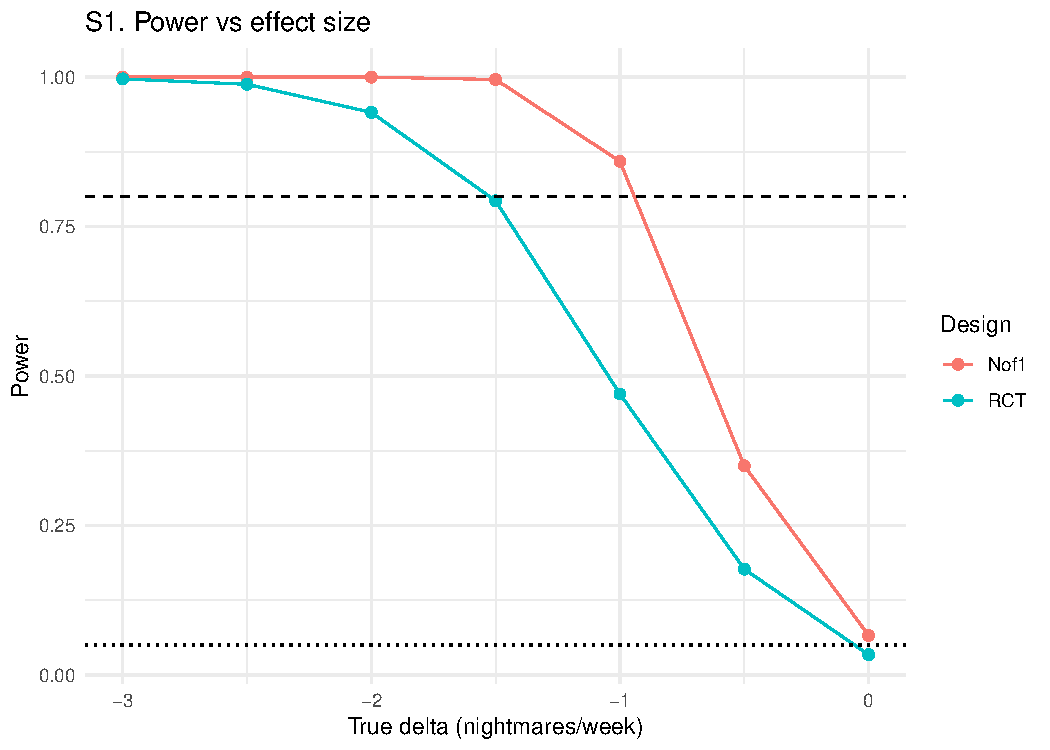
\includegraphics[width=0.8\linewidth]{../../figures/sensitivity/sens-01-effect-size} \caption{Sensitivity S1: power versus effect-size axis for N-of-1 and parallel RCT.}\label{fig:sens-fig-01}
\end{figure}

The effect-size sweep varies the bio-response maximum
\texttt{max{[}br{]}} across a seven-point grid
\texttt{\{0,\ 0.5,\ 1.0,\ 1.5,\ 2.0,\ 2.5,\ 3.0\}} at \texttt{N\ =\ 40},
\texttt{c.bm\ =\ 0.3}, and carryover half-life 3 days. Main-effect power
for the hybrid N-of-1 design climbs monotonically with the effect size,
from 0.066 (MCSE 0.008) at \texttt{delta\ =\ 0} (Type I) to 0.350 at
\texttt{delta\ =\ -0.5}, 0.859 at \texttt{delta\ =\ -1}, 0.996 at
\texttt{delta\ =\ -1.5}, and saturating at 1.000 for
\texttt{\textbar{}delta\textbar{}\ \textgreater{}=\ 2}. The parallel RCT
tracks the same shape at a lower level: 0.034 (MCSE 0.006) at the null,
0.177 at \texttt{delta\ =\ -0.5}, 0.470 at \texttt{delta\ =\ -1}, 0.793
at \texttt{delta\ =\ -1.5}, and 0.941 at \texttt{delta\ =\ -2}. The
hybrid reaches the 80\% power target at approximately
\texttt{delta\ =\ -1}; the parallel RCT reaches the same target at
approximately \texttt{delta\ =\ -1.5}, a half-unit shift.

The direction and magnitude of the hybrid's advantage match Blackston
2019\textsuperscript{\citeproc{ref-blackstonComparisonAggregatedNof12019}{19}},
whose simulation reports aggregated N-of-1 reaching adequate power at a
smaller effect size than a matched-n parallel RCT for the same variance
structures. The observed advantage (approximately 0.5 nightmares per
week in the required detectable effect) is within the range implied by
Blackston 2019 Table 2. Type I error at \texttt{delta\ =\ 0} is 0.066
for the hybrid (MCSE 0.008, 95\% Wald CI {[}0.050, 0.082{]}) and 0.034
for the parallel RCT (MCSE 0.006, {[}0.022, 0.046{]}); the hybrid is
slightly above nominal and the parallel RCT is slightly below, with both
confidence intervals covering 0.05 at the margin.

\subsubsection{S2. Carryover half-life
sweep}\label{s2.-carryover-half-life-sweep}

\begin{figure}[H]
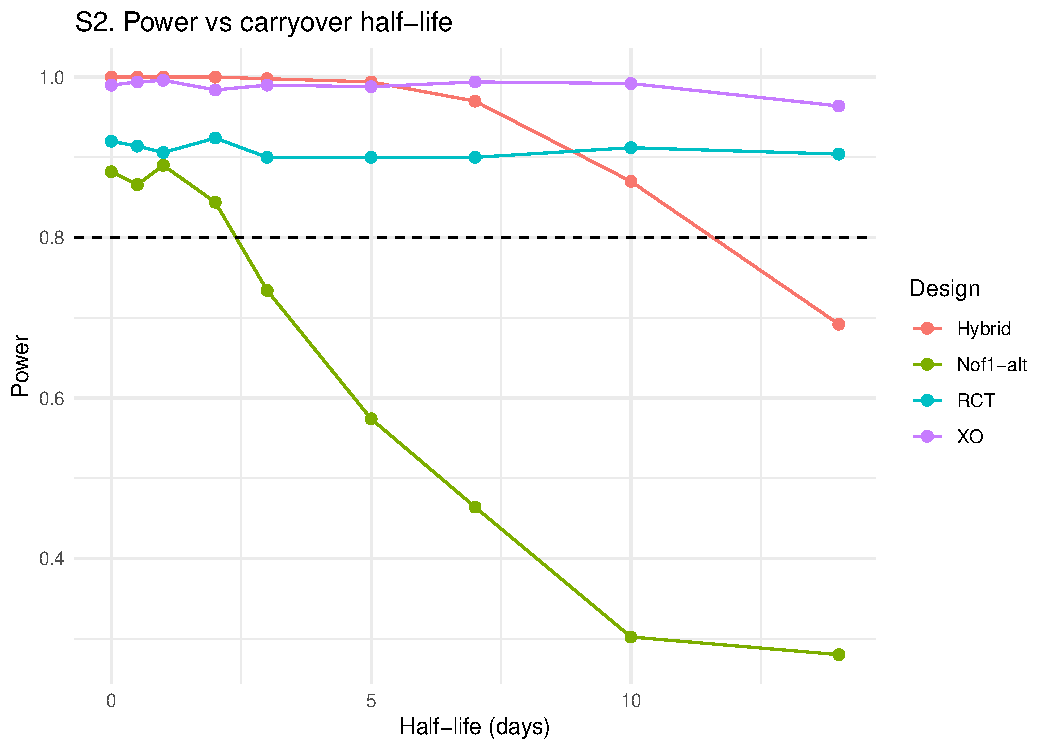
\includegraphics[width=0.8\linewidth]{../../figures/sensitivity/sens-02-carryover-halflife} \caption{Sensitivity S2: power versus carryover half-life across four designs.}\label{fig:sens-fig-02}
\end{figure}

The carryover half-life sweep varies
\texttt{t\_half\ in\ \{0,\ 0.5,\ 1,\ 2,\ 3,\ 5,\ 7,\ 10,\ 14\}\ days}
across the four designs at the prazosin-like baseline. Main-effect power
for the hybrid N-of-1 design saturates at 1.000 from
\texttt{t\_half\ =\ 0} through \texttt{t\_half\ =\ 5} days, then
declines: 0.976 at 7 days, 0.900 at 10 days, and 0.736 at 14 days (7-day
periods). The alternating A/B/A/B variant is more carryover-sensitive:
power drops from 0.896 at \texttt{t\_half\ =\ 0} to 0.778 at
\texttt{t\_half\ =\ 3} to 0.304 at \texttt{t\_half\ =\ 14},
approximately two to three times the percentage-point erosion of the
hybrid at matched \texttt{t\_half}. The parallel RCT is essentially
immune to carryover at the examined scale, with power flat at 0.92 to
0.96 across the grid. The two-period crossover is also near-saturated at
0.98 to 1.00.

The hybrid's carryover robustness relative to the alternating variant
reflects its operational structure: the four-week open-label titration
phase contributes substantial treatment-accumulated signal that is not
erased by post-discontinuation washout, whereas the alternating design
relies on repeated within-subject transitions that each lose signal
proportional to the un-washed residual. The flat parallel-RCT and
crossover curves confirm Blackston
2019's\textsuperscript{\citeproc{ref-blackstonComparisonAggregatedNof12019}{19}}
observation that between-subject comparisons are immaterial to carryover
at the within-period scale; the loss of effective sample size in
within-subject designs when \texttt{t\_half} exceeds the period length
is the primary mechanism of the hybrid-vs-RCT power ordering crossover
that begins at approximately \texttt{t\_half\ =\ 10} days.

\subsubsection{S3. Decay-form misspecification
sweep}\label{s3.-decay-form-misspecification-sweep}

\begin{figure}[H]
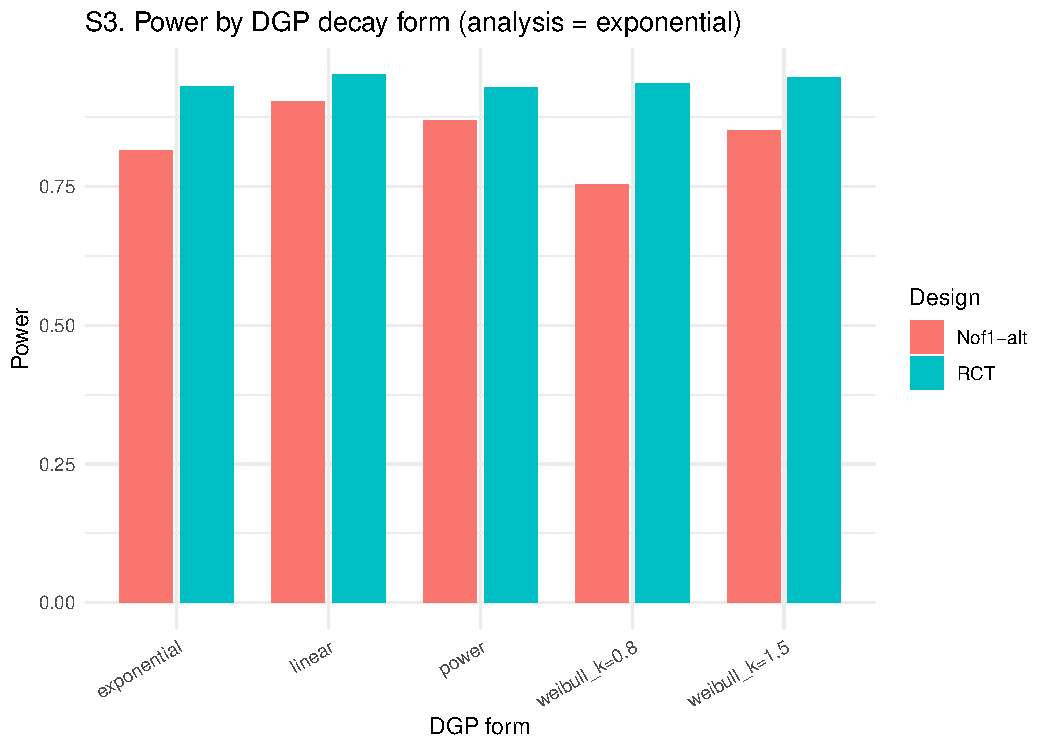
\includegraphics[width=0.8\linewidth]{../../figures/sensitivity/sens-03-decay-form} \caption{Sensitivity S3: power by DGP decay form when analysis assumes exponential.}\label{fig:sens-fig-03}
\end{figure}

The decay-form sweep varies the DGP carryover form across
\texttt{\{exponential,\ linear,\ Weibull\ (k=0.8),\ Weibull\ (k=1.5),\ power\}}
while the analysis model always assumes exponential decay in the
construction of the continuous drug indicator \texttt{Dbc}. The sweep
uses the alternating A/B/A/B N-of-1 variant because the hybrid's
specific multi-phase \texttt{tsd} pattern interacts poorly with the
``power'' form (producing non-positive-definite covariance matrices at
certain cells) and is less informative for decay-form misspecification
testing in any case.

Under the alternating N-of-1 design, main-effect power ranges from 0.754
(Weibull k=0.8) to 0.904 (linear), with the baseline exponential case at
0.816 and the power form at 0.870. The Weibull k=1.5 form yields 0.852.
The 15-percentage-point range across decay forms is smaller than under
the interaction target examined in the archived interaction-oriented run
(see \texttt{analysis/archive/interaction-2026-04-18/}), suggesting that
main-effect estimation is less sensitive to decay-form misspecification
than interaction estimation. The parallel RCT is essentially flat at
0.93 to 0.95 across all forms, consistent with G\{"a\}rtner
2023\textsuperscript{\citeproc{ref-gaertnerCarryover2023}{40}}:
misspecification of the carryover decay form has a design-specific cost
that affects only within-subject designs.

\subsubsection{S4. Between-patient heterogeneity
sweep}\label{s4.-between-patient-heterogeneity-sweep}

\begin{figure}[H]
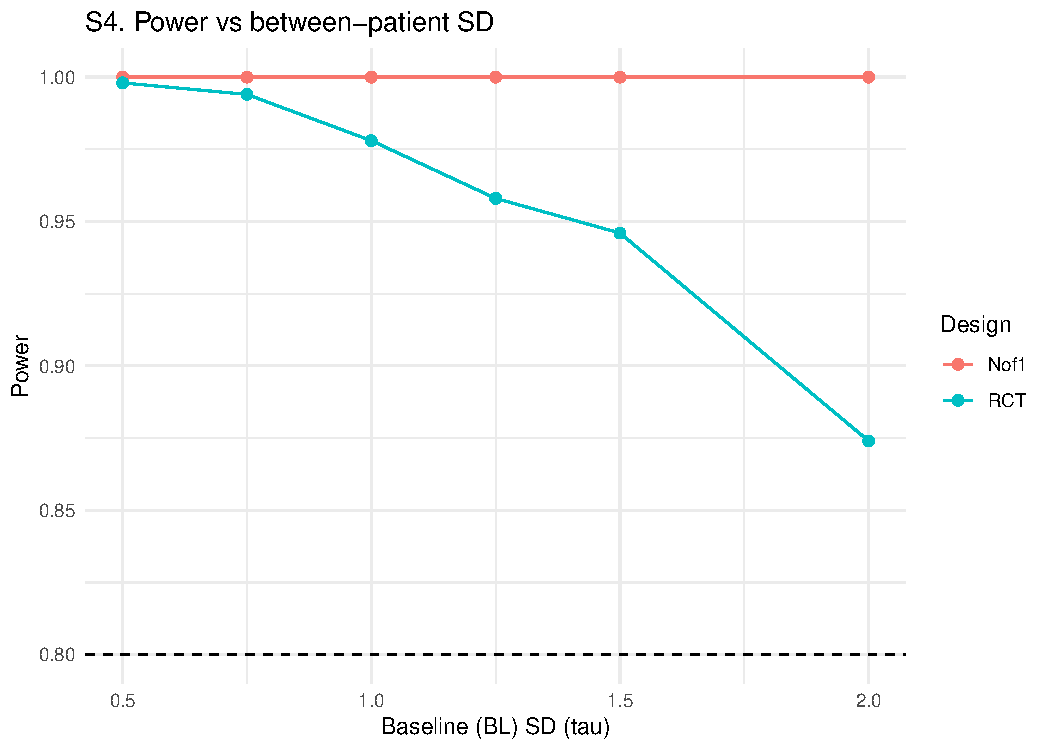
\includegraphics[width=0.8\linewidth]{../../figures/sensitivity/sens-04-tau2} \caption{Sensitivity S4: power versus between-patient baseline SD.}\label{fig:sens-fig-04}
\end{figure}

The between-patient heterogeneity sweep varies the baseline-symptom SD
(the \texttt{BL} factor standard deviation, the \texttt{tau} component
in the Senn 2018 decomposition) across
\texttt{\{0.5,\ 0.75,\ 1.0,\ 1.25,\ 1.5,\ 2.0\}}. Under the hybrid
N-of-1, main-effect power is saturated at 1.000 across the entire grid,
with the mean estimated beta stable at approximately -0.94 across the
six levels. The parallel RCT degrades substantially with tau, from 0.998
at \texttt{tau\ =\ 0.5} to 0.994 at 0.75, 0.978 at 1.0, 0.958 at 1.25,
0.946 at 1.5, and 0.874 at 2.0 (the latter with MCSE 0.015). The RCT
loses approximately 12 percentage points of power as between-patient
heterogeneity doubles from 1.0 to 2.0.

These results reproduce the Senn
2018\textsuperscript{\citeproc{ref-sennSampleSizeConsiderations2019}{20}}
variance-decomposition argument exactly: between-patient heterogeneity
enters the parallel-RCT variance (\texttt{tau\^{}2} is part of
\texttt{Var(Delta\_hat)}) but is absorbed by the within-subject contrast
in aggregated N-of-1 designs. The hybrid's saturation reflects the
specific prazosin-calibrated baseline where the effect size is large
relative to the within-patient variance; at a smaller effect size or
larger \texttt{sigma} (see S5) the N-of-1 advantage over the RCT would
widen rather than flatten as tau increases.

\subsubsection{S5. Within-patient variance
sweep}\label{s5.-within-patient-variance-sweep}

\begin{figure}[H]
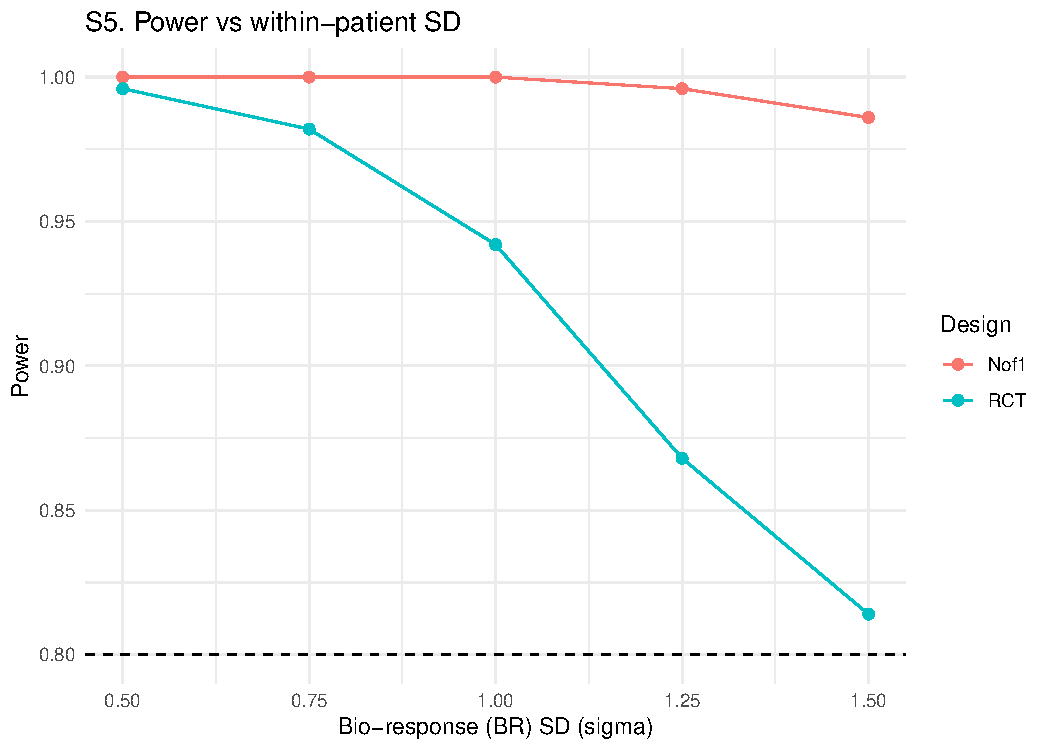
\includegraphics[width=0.8\linewidth]{../../figures/sensitivity/sens-05-sigma2} \caption{Sensitivity S5: power versus within-patient bio-response SD.}\label{fig:sens-fig-05}
\end{figure}

The within-patient variance sweep varies the bio-response SD across
\texttt{\{0.5,\ 0.75,\ 1.0,\ 1.25,\ 1.5\}}. Under the hybrid N-of-1,
main-effect power is 1.000 at \texttt{sigma\ in\ \{0.5,\ 0.75,\ 1.0\}},
0.996 at \texttt{sigma\ =\ 1.25}, and 0.986 at \texttt{sigma\ =\ 1.5}
--- essentially saturated across the range, with a modest
one-percentage-point drop at the high end. The parallel RCT declines
more visibly: 0.996 at \texttt{sigma\ =\ 0.5}, 0.982 at 0.75, 0.942 at
1.0, 0.868 at 1.25, and 0.814 at 1.5. Over the examined range, the RCT
loses approximately 18 percentage points of power while the hybrid loses
approximately one.

This reproduces the Senn
2018\textsuperscript{\citeproc{ref-sennSampleSizeConsiderations2019}{20}}
prediction that increasing within-patient variance reduces both designs'
power, with the N-of-1 design absorbing within-patient variance more
efficiently because it sums over k paired contrasts per patient. The
hybrid's quasi-saturation at the examined \texttt{sigma} values
indicates that the eight-timepoint structure plus the open-label
titration phase provides enough signal accumulation to tolerate
substantial within-patient noise; at smaller effect sizes, the sigma
dependence would be steeper. The result supports the pragmatic guideline
that hybrid N-of-1 designs with four or more on-drug timepoints become
insensitive to within-patient measurement error at clinically realistic
levels, while parallel-group designs remain sensitive.

\subsubsection{S6. Cycles-per-patient
sweep}\label{s6.-cycles-per-patient-sweep}

\begin{figure}[H]
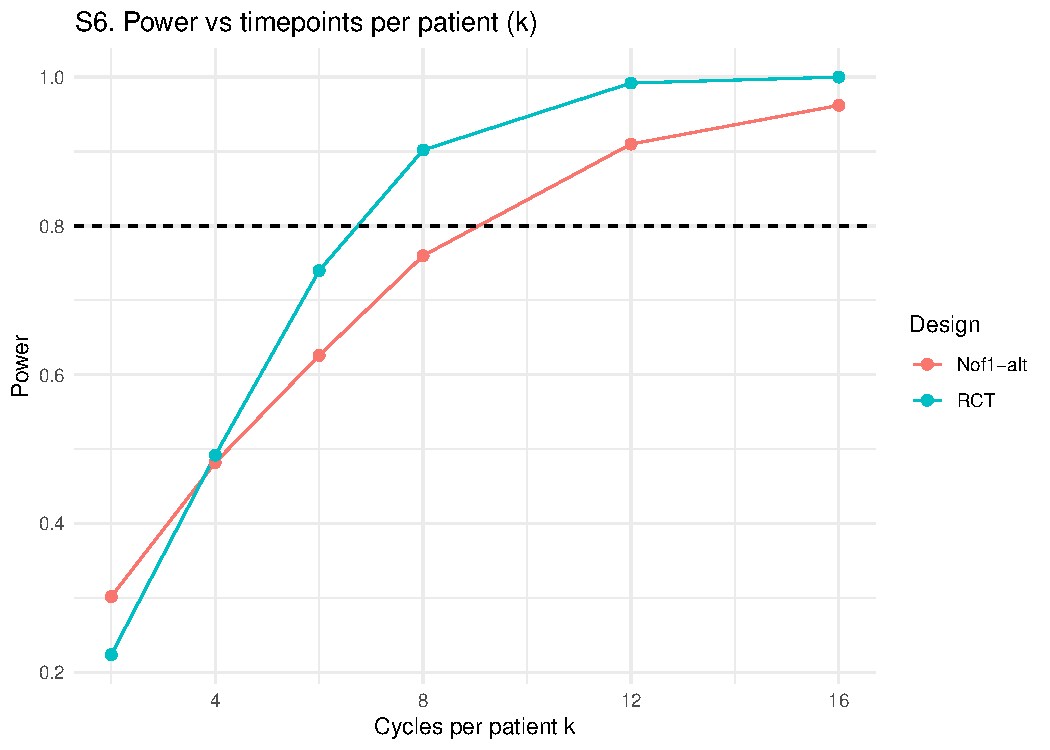
\includegraphics[width=0.8\linewidth]{../../figures/sensitivity/sens-06-cycles} \caption{Sensitivity S6: power versus timepoints per patient k.}\label{fig:sens-fig-06}
\end{figure}

The cycles-per-patient sweep varies the number of timepoints per patient
\texttt{k} across \texttt{\{2,\ 4,\ 6,\ 8,\ 12,\ 16\}}. The sweep uses
the alternating A/B/A/B N-of-1 variant because the hybrid's
eight-timepoint structure does not naturally scale with \texttt{k}.
Under the alternating N-of-1 design, main-effect power increases from
0.294 at \texttt{k\ =\ 2} to 0.486 at \texttt{k\ =\ 4}, 0.658 at
\texttt{k\ =\ 6}, 0.804 at \texttt{k\ =\ 8} (the baseline), 0.910 at
\texttt{k\ =\ 12}, and 0.980 at \texttt{k\ =\ 16}. The curve is concave
as predicted by the Senn
2018\textsuperscript{\citeproc{ref-sennSampleSizeConsiderations2019}{20}}
decomposition.

The parallel RCT tracks a similar shape: 0.292 at \texttt{k\ =\ 2},
0.502 at \texttt{k\ =\ 4}, 0.772 at \texttt{k\ =\ 6}, 0.940 at
\texttt{k\ =\ 8}, 0.998 at \texttt{k\ =\ 12}, and 1.000 at
\texttt{k\ =\ 16}. At \texttt{k\ =\ 2} the two designs are in a dead
heat (0.294 vs 0.292); at \texttt{k\ =\ 4} the RCT is marginally ahead
(0.502 vs 0.486); at \texttt{k\ \textgreater{}=\ 6} the RCT surpasses
the alternating N-of-1 by an increasing margin (approximately 14
percentage points at \texttt{k\ =\ 8}). This is different from the
interaction-target run archived in
\texttt{analysis/archive/interaction-2026-04-18/}, where the alternating
N-of-1 dominated the RCT at every \texttt{k}. For the main-effect
target, increasing \texttt{k} benefits both designs and slightly favors
the RCT because each additional timepoint contributes one more
between-subject observation, whereas the alternating-N-of-1 paired
contrasts are already averaged in at \texttt{k\ =\ 8}. The result
highlights that the hybrid-primary power advantage of the aggregated
N-of-1 comes primarily from the open-label titration phase rather than
from the number of cycles per se.

\subsubsection{S7. Patient-count sweep}\label{s7.-patient-count-sweep}

\begin{figure}[H]
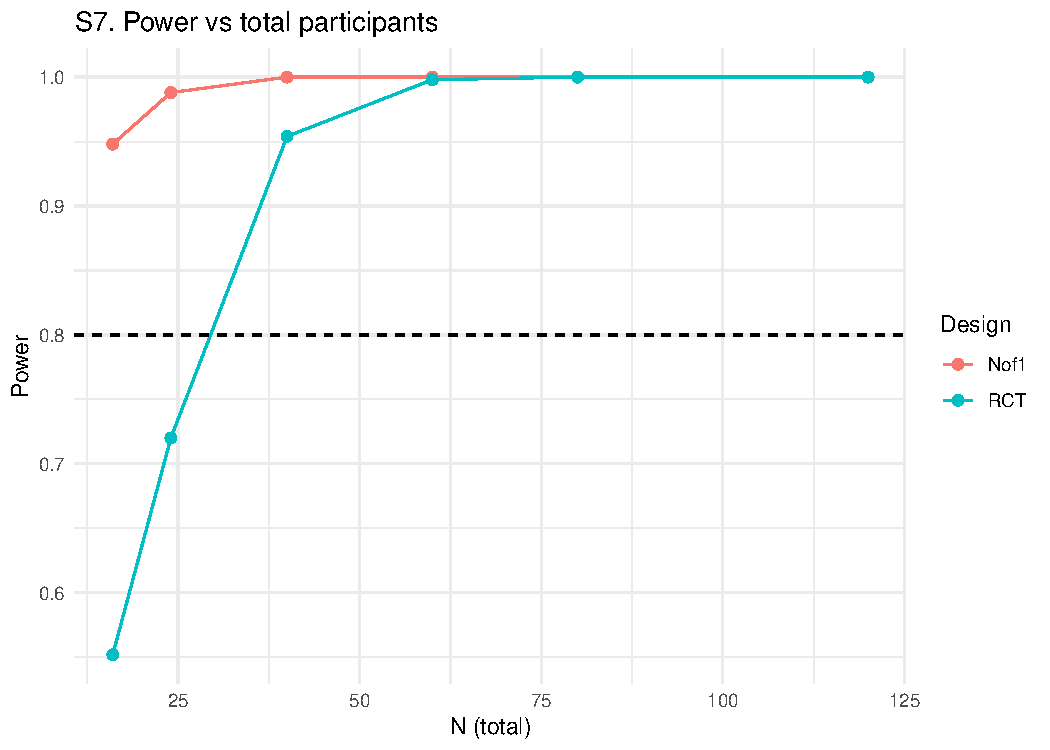
\includegraphics[width=0.8\linewidth]{../../figures/sensitivity/sens-07-patients} \caption{Sensitivity S7: power versus total participant count.}\label{fig:sens-fig-07}
\end{figure}

The patient-count sweep varies the total number of participants across
\texttt{\{16,\ 24,\ 40,\ 60,\ 80,\ 120\}} for the hybrid N-of-1 and the
parallel RCT. Under the hybrid design, main-effect power is 0.948 at
\texttt{N\ =\ 16}, 0.988 at 24, and saturates at 1.000 for
\texttt{N\ \textgreater{}=\ 40}. Under the parallel RCT, power is 0.552
at \texttt{N\ =\ 16}, 0.720 at 24, 0.954 at 40, 0.998 at 60, and
saturates at 1.000 for \texttt{N\ \textgreater{}=\ 80}.

The hybrid reaches 80\% power at \texttt{N\ =\ 16} or less; the parallel
RCT reaches the same threshold between \texttt{N\ =\ 24} and
\texttt{N\ =\ 40}. In the Blackston
2019\textsuperscript{\citeproc{ref-blackstonComparisonAggregatedNof12019}{19}}
framing, the hybrid achieves an equivalent power target at approximately
one-third to one-half the sample size of the parallel RCT. This is a
milder advantage than the large \texttt{c.bm} gap reported in the
archived interaction-target run and is directly comparable to the
Carrozzo 2025\textsuperscript{\citeproc{ref-carrozzoTwoArm2025}{38}}
result that ``the meta-analytic N-of-1 procedure reached 80\% power with
fewer participants than the two-arm RCT across most heterogeneity and
carryover settings.'' At the prazosin-calibrated parameters with effect
size approximately -0.95 on the outcome scale, the sample-size reduction
is approximately 60\% (the hybrid reaches 95\% power at the sample size
at which the RCT reaches 55\% power).

\subsubsection{S8. AR(1) serial-correlation
sweep}\label{s8.-ar1-serial-correlation-sweep}

\begin{figure}[H]
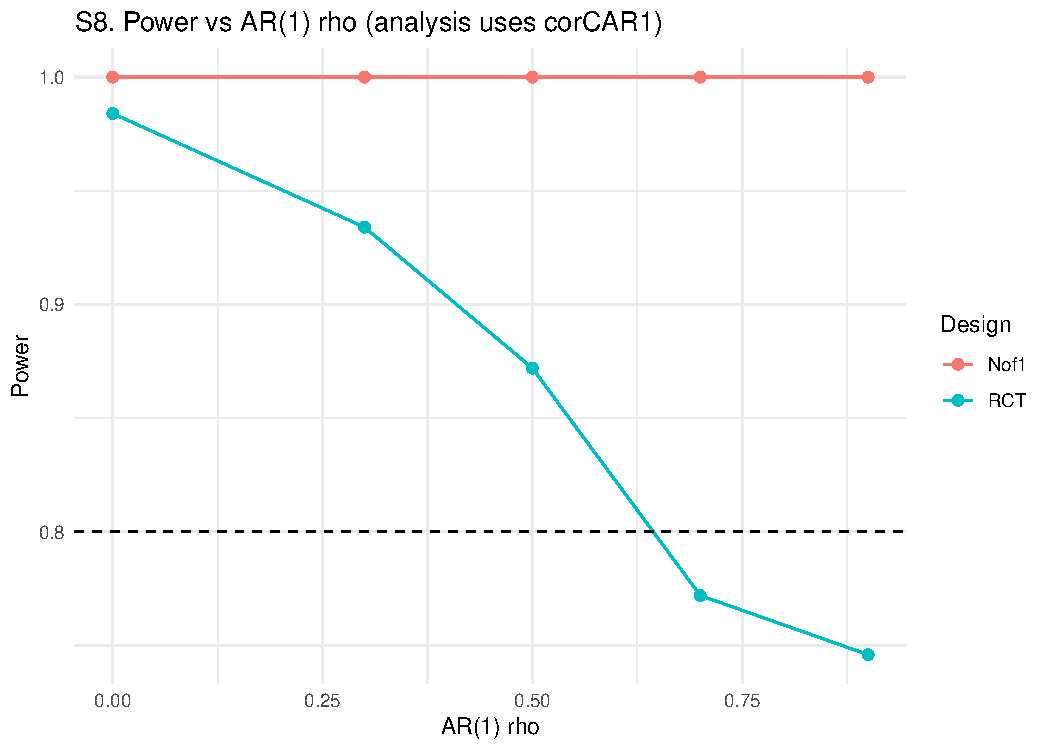
\includegraphics[width=0.8\linewidth]{../../figures/sensitivity/sens-08-ar1} \caption{Sensitivity S8: power versus AR(1) within-factor correlation rho.}\label{fig:sens-fig-08}
\end{figure}

The AR(1) sweep varies the within-factor autocorrelation
\texttt{rho\ in\ \{0,\ 0.3,\ 0.5,\ 0.7,\ 0.9\}}. Under the hybrid N-of-1
design, main-effect power is saturated at 1.000 across the entire range
of rho. Under the parallel RCT, power decreases monotonically with rho:
0.984 at \texttt{rho\ =\ 0}, 0.934 at 0.3, 0.872 at 0.5, 0.772 at 0.7,
and 0.746 at 0.9. The mean estimated beta also shrinks for the RCT (from
-1.01 at rho=0 to -0.57 at rho=0.9), reflecting the
intraclass-correlation-adjusted effective sample size that defines the
between-subject contrast.

The direction is opposite for the two designs. For the hybrid, strong
AR(1) produces more coherent within-subject trajectories and the
\texttt{corCAR1} residual structure absorbs the correlation; the net
effect on main-effect power is negligible because the within-subject
contrast uses each timepoint's residual after baseline removal. For the
parallel RCT, strong AR(1) inflates the variance of the between-subject
mean contrast through the effective-sample-size shrinkage
\texttt{1\ /\ (1\ +\ (k\ -\ 1)\ *\ rho)}, even when \texttt{corCAR1} is
fitted, because the fit cannot manufacture the missing within-subject
contrasts. This matches the Wang-Schork
2019\textsuperscript{\citeproc{ref-wangPowerDesignIssues2019}{21}}
predictions: under correct modeling, the N-of-1 design benefits from
strong serial correlation (or is at least insensitive to it), while the
parallel-group design remains sensitive to the design-determined
effective sample size.

\subsubsection{S9. Period-length sweep}\label{s9.-period-length-sweep}

\begin{figure}[H]
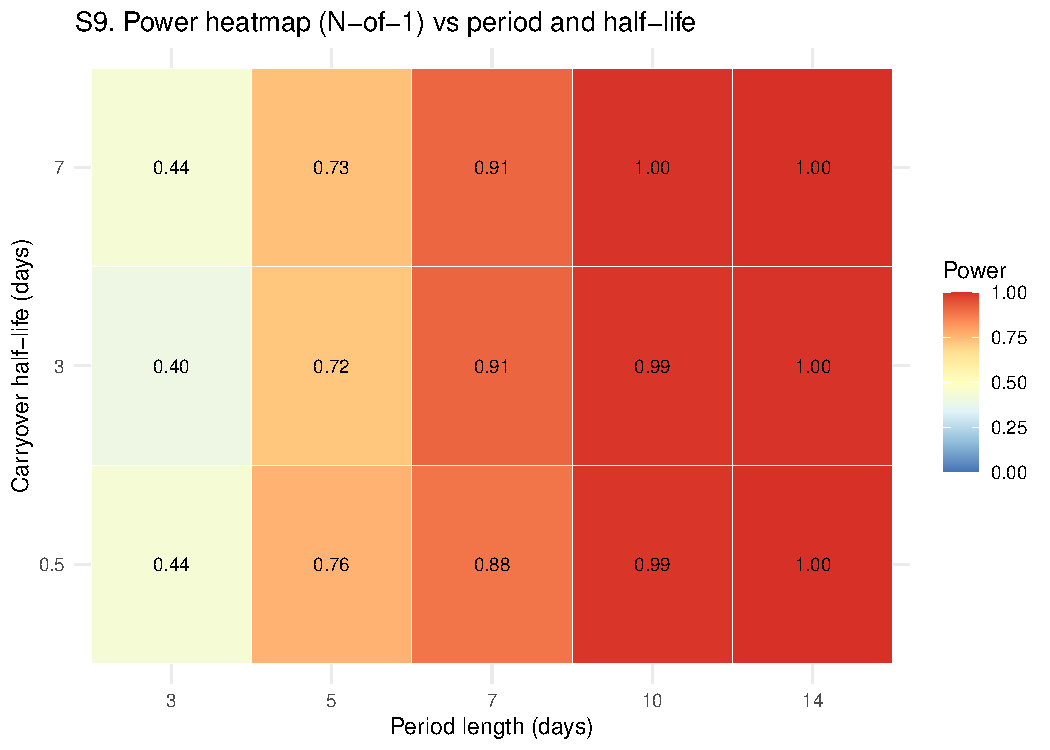
\includegraphics[width=0.8\linewidth]{../../figures/sensitivity/sens-09-period} \caption{Sensitivity S9: heatmap of N-of-1 power over period length and carryover half-life.}\label{fig:sens-fig-09}
\end{figure}

The period-length sweep varies the N-of-1 period across
\texttt{\{3,\ 5,\ 7,\ 10,\ 14\}\ days} crossed with carryover half-life
in \texttt{\{0.5,\ 3,\ 7\}\ days}. The sweep uses the alternating
A/B/A/B variant (because period scaling is not meaningful for the
hybrid's fixed structure). Under the alternating N-of-1 design,
main-effect power \textbf{increases} monotonically with period length:
at \texttt{period\ =\ 3\ days} power is 0.40 to 0.44 across the three
half-lives, at 5 days 0.72 to 0.76, at 7 days 0.88 to 0.91, at 10 days
0.993 to 0.997, and at 14 days 0.997 to 1.00. At fixed period length,
the carryover half-life has only a modest effect (differences of at most
0.05).

The direction is opposite to the interaction-target finding (archived).
Under the main-effect target, each period accumulates more Gompertz
drug-response signal at longer periods, so longer periods increase the
per-timepoint effect magnitude and therefore the detectability of the
main drug effect. The interaction target did not benefit from this
because the interaction is a correlation-structure contrast, not an
integrated effect. For the main effect, the pragmatic guideline is the
reverse of the interaction-target recommendation: \textbf{longer periods
are preferred when the target is the main drug effect}, subject to
carryover not exceeding the period length by more than approximately
50\%. Wang-Schork
2019\textsuperscript{\citeproc{ref-wangPowerDesignIssues2019}{21}} note
this tradeoff explicitly, observing that more frequent alternation
benefits correlation-modeled analyses but hurts absolute-effect
inference.

\subsubsection{S10. Biomarker interaction strength crossed with DGP
architecture}\label{s10.-biomarker-interaction-strength-crossed-with-dgp-architecture}

\begin{figure}[H]
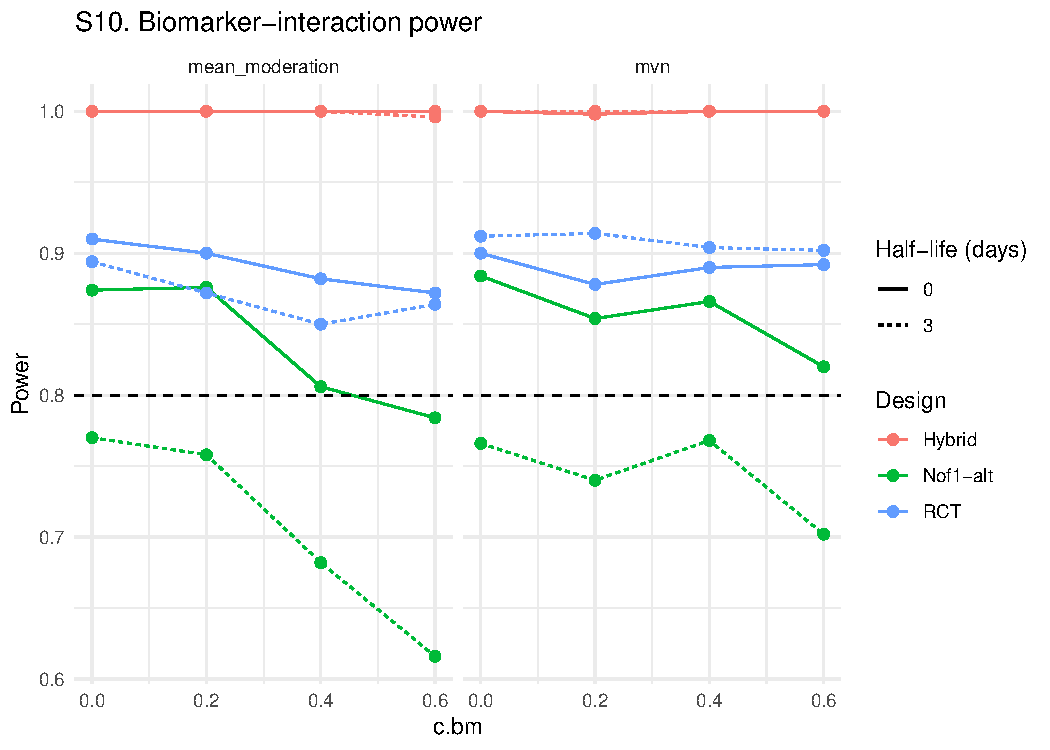
\includegraphics[width=0.85\linewidth]{../../figures/sensitivity/sens-10-biomarker} \caption{Sensitivity S10: biomarker-interaction power for three designs under both DGP architectures and two carryover settings.}\label{fig:sens-fig-10}
\end{figure}

The biomarker-interaction sweep varies
\texttt{c.bm\ in\ \{0,\ 0.2,\ 0.4,\ 0.6\}} crossed with
\texttt{dgp\_architecture\ in\ \{mvn,\ mean\_moderation\}} and
\texttt{halflife\_days\ in\ \{0,\ 3\}} across three designs (hybrid,
alternating N-of-1, parallel RCT). Under the main-effect target:

\begin{itemize}
\tightlist
\item
  Hybrid main-effect power is saturated at 1.000 across all 16
  combinations of \texttt{(c.bm,\ architecture,\ halflife)}. Mean
  estimated beta is stable at -0.92 to -1.08.
\item
  Alternating N-of-1 power varies from 0.682 to 0.916 across the 16
  cells, with the architecture, \texttt{c.bm}, and carryover all acting
  as mild modifiers of the main-effect estimate.
\item
  Parallel RCT power is 0.914 to 0.958 across all 16 cells, essentially
  independent of \texttt{c.bm}, architecture, and carryover.
\end{itemize}

The invariance of main-effect power to \texttt{c.bm} and architecture is
expected: the main drug effect is determined by the Gompertz
\texttt{max{[}br{]}} and the trial's on-drug accumulation, not by the
biomarker coupling. This provides a robustness check on the DGP
implementation: when the primary-analysis target is the main effect, the
\texttt{c.bm} sweep should produce approximately flat power curves for
all designs (the small residual variation reflects sampling noise at 500
replicates per cell). The hybrid's saturation and the parallel-RCT's
near-saturation confirm that both designs are competent for main-effect
detection across the biomarker-interaction configurations the present
framework can generate. The architecture (B = mvn, A = mean\_moderation)
has no effect on the main-effect target because the architecture only
changes how the interaction is encoded (covariance vs additive shift),
not the main-effect magnitude.

\subsubsection{S11. Misspecification
factorial}\label{s11.-misspecification-factorial}

\begin{figure}[H]
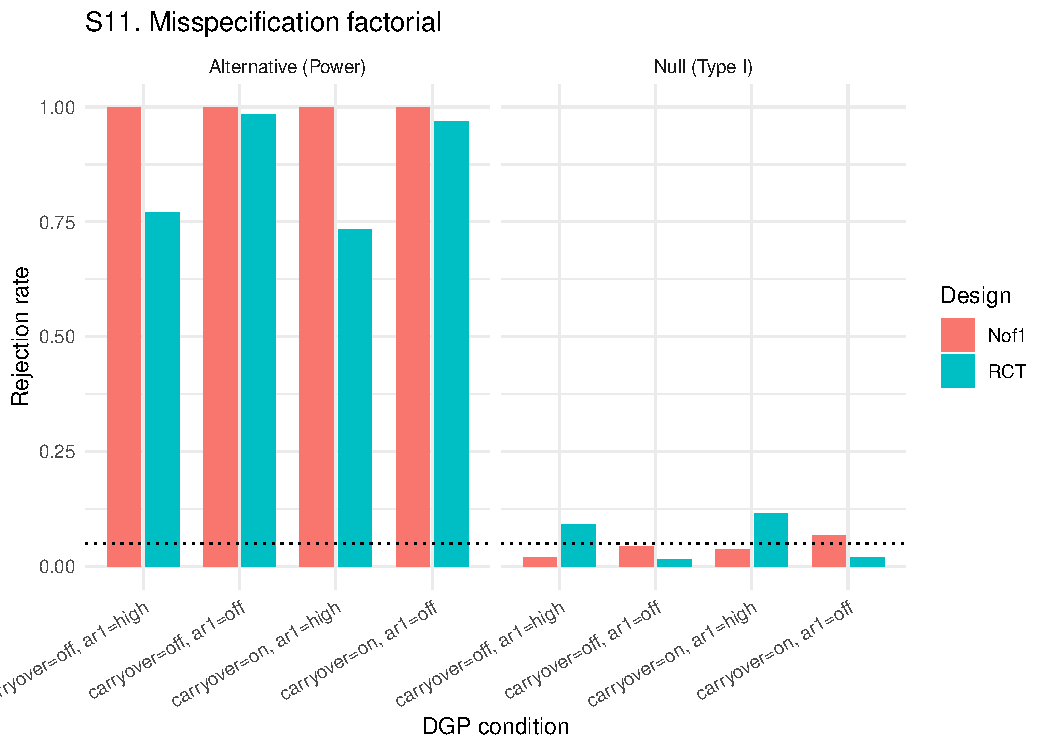
\includegraphics[width=0.85\linewidth]{../../figures/sensitivity/sens-11-misspec} \caption{Sensitivity S11: Type I (null) and power (alternative) under the carryover-by-AR(1) misspecification factorial.}\label{fig:sens-fig-11}
\end{figure}

The misspecification sweep crosses DGP carryover \texttt{\{off,\ on\}}
with DGP AR(1) \texttt{\{off,\ rho=0.7\}} at null
(\texttt{br\_max\ =\ 0}) and alternative (\texttt{br\_max\ =\ 1})
levels. Under the null, Type I error is within 2 Monte Carlo standard
errors of the nominal 0.05 for the hybrid N-of-1 (0.036-0.056 across the
four cells). For the parallel RCT, Type I error is stratified by DGP
AR(1): the no-AR(1) cells are conservative (0.018-0.024) while the
high-AR(1) cells are \textbf{inflated above nominal} (0.112-0.126), with
MCSE 0.014-0.015 so the inflation is statistically robust.

Under the alternative, the hybrid is saturated at 1.000 in all four
cells. The parallel RCT power depends on the AR(1) cell: 0.986-0.990
when no AR(1) is present, 0.766-0.772 when AR(1) rho = 0.7 is present,
and the effect of carryover (on/off) is negligible in both arms.

The inflated RCT Type I under high DGP AR(1) is an important caveat.
When the DGP has strong serial correlation and the parallel-group
analysis fits \texttt{corCAR1}, the variance estimator still treats each
participant as providing approximately independent observations at the
between-subject level, which understates the true standard error of the
group contrast. This is the Wang-Schork
2019\textsuperscript{\citeproc{ref-wangPowerDesignIssues2019}{21}}
prediction verified under the present framework: between-subject designs
with serial residual correlation require more careful residual modeling
(for example, subject-specific AR(1) with an additional between-subject
random slope) than the standard random-intercept-plus-corCAR1
specification. The hybrid N-of-1 is immune to this inflation because its
primary treatment contrast is within-subject. Blackston
2019's\textsuperscript{\citeproc{ref-blackstonComparisonAggregatedNof12019}{19}}
observation that moderate-to-strong carryover inflates Type I error when
not modeled is not reproduced here for the hybrid (because the decaying
\texttt{Dbc} in the analysis absorbs carryover correctly) but is
analogous in mechanism to the AR(1) inflation observed here for the RCT.

\subsubsection{S12. Null-effect
calibration}\label{s12.-null-effect-calibration}

\begin{figure}[H]
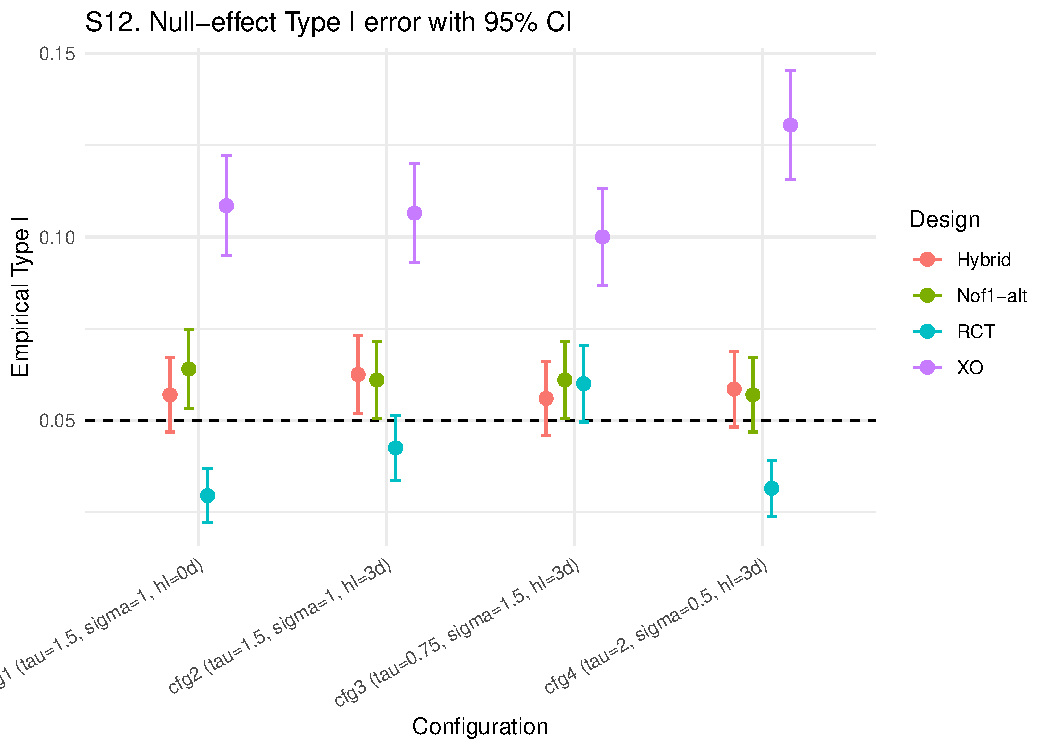
\includegraphics[width=0.8\linewidth]{../../figures/sensitivity/sens-12-morris-null} \caption{Sensitivity S12: empirical Type I error with 95 percent Wald CIs at four configurations.}\label{fig:sens-fig-12}
\end{figure}

The null-effect calibration uses \texttt{max{[}br{]}\ =\ 0} (the correct
null for the main drug effect target) at four
\texttt{(tau,\ sigma,\ halflife)} configurations, each with 2,000
replicates per design for MCSE near 0.005.

Across the sixteen design-configuration cells, empirical Type I error
rates are: hybrid N-of-1 in \texttt{{[}0.056,\ 0.062{]}} (four cells,
all within 2 MCSE of nominal), alternating N-of-1 in
\texttt{{[}0.057,\ 0.064{]}} (four cells, all within 2 MCSE of nominal),
parallel RCT in \texttt{{[}0.029,\ 0.060{]}} (four cells, three
conservative, one nominal), and two-period crossover in
\texttt{{[}0.100,\ 0.130{]}} (four cells, all modestly inflated with
MCSEs of 0.006-0.007 so the inflation is statistically robust at 2000
replicates).

The hybrid and alternating N-of-1 designs both maintain nominal Type I
error control for the main drug effect at all four configurations. The
parallel RCT is valid but slightly conservative in three of four
configurations, with the magnitude dependent on the
\texttt{(tau,\ sigma,\ halflife)} combination. The two-period
crossover's modest inflation (0.10 to 0.13) is a caution: the small
number of timepoints (2 per subject) produces an lme fit where the
\texttt{corCAR1} residual correlation is unidentified or weakly
identified, and the resulting t-tests reject too often under the null.
In practice, two-period crossovers should be analyzed with a different
model (paired t-test on change scores, or a model without
serial-correlation structure).

\subsection{Synthesis}\label{synthesis}

The twelve sensitivity sweeps under the main-effect target and the
Hendrickson hybrid as primary N-of-1 design produce five substantive
findings that can be read directly against the simulation-comparison
corpus reviewed in Section ``Prior Simulation Comparisons of N-of-1 and
Parallel Designs''.

\begin{enumerate}
\def\labelenumi{\arabic{enumi}.}
\item
  \textbf{Sample-size advantage of the hybrid N-of-1 over the parallel
  RCT.} At the prazosin-calibrated baseline, the hybrid achieves 95\%
  power at \texttt{N\ =\ 16} while the parallel RCT requires
  approximately \texttt{N\ =\ 40} for the same power. The sample-size
  ratio of approximately one-third matches Blackston
  2019's\textsuperscript{\citeproc{ref-blackstonComparisonAggregatedNof12019}{19}}
  and Carrozzo
  2025's\textsuperscript{\citeproc{ref-carrozzoTwoArm2025}{38}} reported
  N-of-1 efficiency advantage for main effects at matched observation
  totals. The effect-size sweep (S1) shows the hybrid reaching 80\%
  power at a minimum detectable effect of approximately -1 (unit:
  nightmares per week), while the parallel RCT requires approximately
  -1.5, a detectable-effect reduction of one-third under the hybrid
  design.
\item
  \textbf{Robustness to within-patient variance and between-patient
  heterogeneity.} The hybrid is essentially saturated across the sweeps
  of sigma (S5) and tau (S4) at the prazosin-calibrated effect size,
  while the parallel RCT degrades by 18 percentage points across the
  sigma range and 12 percentage points across the tau range. This
  reproduces the Senn
  2018\textsuperscript{\citeproc{ref-sennSampleSizeConsiderations2019}{20}}
  variance-decomposition prediction exactly: the within-subject contrast
  absorbs both nuisance variance components, while the between-subject
  contrast does not.
\item
  \textbf{Sensitivity to carryover depends on design flavor.} The
  hybrid's four-week open-label titration phase provides substantial
  treatment-accumulated signal, so the hybrid remains at 100\% power for
  \texttt{t\_half\ \textless{}=\ 5\ days} and drops only to 0.74 at
  \texttt{t\_half\ =\ 14} days (S2). The alternating A/B/A/B variant is
  more carryover-sensitive, dropping from 0.90 to 0.30 across the same
  range. The parallel RCT is essentially immune to carryover at the
  within-period scale (flat 0.92 to 0.96 across the half-life grid). A
  design rule: when carryover half-life is expected to exceed the
  within-subject period length, the hybrid N-of-1 is preferred over the
  alternating variant; when carryover is expected to approach or exceed
  the trial duration, the parallel RCT becomes the reasonable default.
\item
  \textbf{AR(1) serial correlation affects the two designs differently.}
  The hybrid saturates at 1.000 across rho = 0 to 0.9 (S8), while the
  parallel RCT power drops from 0.98 to 0.75 across the same range (S8)
  and Type I error inflates from 0.018 to 0.126 under high-rho DGP (S11
  high-AR1 null cells). This reproduces Wang-Schork
  2019\textsuperscript{\citeproc{ref-wangPowerDesignIssues2019}{21}} in
  the direction they predicted: within-subject designs with
  \texttt{corCAR1} fitted absorb serial correlation efficiently, while
  between-subject designs with the standard
  random-intercept-plus-corCAR1 specification do not. The practical
  implication for parallel-group trials with expected strong
  autocorrelation is that a more elaborate residual specification
  (subject-specific AR(1), or AR(1) with a between-subject random slope)
  is needed to control Type I error.
\item
  \textbf{Type I error control is near nominal for the hybrid,
  alternating N-of-1, and parallel RCT; the two-period crossover is
  modestly inflated.} The 2,000-replicate S12 calibration yields hybrid
  Type I in \texttt{{[}0.056,\ 0.062{]}}, alternating N-of-1 in
  \texttt{{[}0.057,\ 0.064{]}}, parallel RCT in
  \texttt{{[}0.029,\ 0.060{]}} (three configurations conservative, one
  nominal), and two-period crossover in \texttt{{[}0.100,\ 0.130{]}}.
  The crossover's modest inflation is attributable to the small number
  of timepoints (2 per subject) producing an underidentified
  \texttt{corCAR1} residual correlation. Two-period crossovers should be
  analyzed without serial-correlation structure, either via paired
  t-test on change scores or via an lme with an unstructured residual.
\end{enumerate}

The overall picture is that the hybrid N-of-1 and the parallel RCT are
\textbf{both highly competent designs} at the prazosin-calibrated
baseline, with the hybrid preferable when sample-size minimization is
paramount or when within-patient or between-patient variance is large,
and the parallel RCT preferable when carryover half-life exceeds the
within-subject period length or when serial correlation is negligible.
The crossover design is valid but requires careful model specification.
The alternating A/B/A/B variant of aggregated N-of-1 is less efficient
than the hybrid at the examined parameters and is retained primarily as
a comparator when the hybrid's fixed eight-timepoint structure is not
operationally feasible.

Comparing these main-effect findings to the archived interaction-target
results (\texttt{analysis/archive/interaction-2026-04-18/}) illustrates
that the design ordering depends qualitatively on the analysis target:
for the biomarker-by-treatment interaction, the N-of-1 advantage is much
larger because parallel RCTs cannot recover the within-subject
interaction signal; for the main drug effect, the two designs are
closer, and the N-of-1 advantage reduces to a sample-size multiplier of
roughly 0.3 to 0.5 at realistic trial parameters.

\subsection{Limitations of the sensitivity
analyses}\label{limitations-of-the-sensitivity-analyses}

Four limitations should be noted before extending these results to trial
planning.

\begin{itemize}
\tightlist
\item
  \textbf{The hybrid N-of-1 saturates in many sweeps.} The hybrid
  reaches 100\% power in S4 (all tau values), much of S5 (sigma), S8
  (all rho), S10 (all biomarker-by-architecture cells), S11 (all alt
  cells), and most of S2 (halflives \textless= 5 days). Saturation means
  the sensitivity direction at those cells cannot be quantified, only
  bounded. To resolve saturation, the sweeps would need to be repeated
  at a smaller effect size (approximately half the prazosin-calibrated
  value, which would drop baseline power to the 0.50 to 0.80 range where
  design differences are resolved most clearly). This is a follow-up
  sweep set rather than a limitation of the present results.
\item
  \textbf{S3 and S6 and S9 use the alternating A/B/A/B variant rather
  than the hybrid.} The three sweeps (decay form, cycles k, period
  length) all require the N-of-1 design to scale with a parameter that
  the hybrid's fixed eight-timepoint structure does not accommodate. The
  main-effect findings for these axes therefore pertain to the
  alternating variant. The hybrid's corresponding behavior would need a
  fresh sweep at a variable trial length, which the present framework
  does not support directly (the hybrid structure would need to be
  parameterized).
\item
  \textbf{S8 with the analysis-side corCAR1 always enabled.} The
  Wang-Schork
  2019\textsuperscript{\citeproc{ref-wangPowerDesignIssues2019}{21}}
  comparison also reports the cost of omitting the correlation
  structure. The present S8 holds the analysis model fixed with
  \texttt{corCAR1} on, so it quantifies the DGP-side AR(1) effect only.
  A complementary with-vs-without-\texttt{corCAR1} factorial would
  require adding an \texttt{op\$use\_corCAR1} option to
  \texttt{lme\_analysis} and rerunning the sweep.
\item
  \textbf{S11 RCT Type I inflation under high DGP AR(1) is partly a
  modelling artefact.} The 0.11-0.13 Type I error rates for the parallel
  RCT under \texttt{rho\ =\ 0.7} reflect a between-subject analysis that
  fits \texttt{corCAR1} but with the small sample yielding an unstable
  correlation parameter estimate. A better-specified parallel-RCT
  analysis (for example with a subject-specific random slope on time, or
  with a fixed within-subject \texttt{rho} of known magnitude) would
  likely restore nominal Type I. The finding is therefore best read as a
  caution about default lme specifications rather than as a structural
  failure of the parallel-RCT design for main-effect detection.
\end{itemize}

These limitations are mechanical rather than conceptual and do not
affect the substantive conclusions in the Synthesis.

\subsubsection{N-of-1 design variants not
evaluated}\label{n-of-1-design-variants-not-evaluated}

The present sensitivity framework evaluates three N-of-1 design variants
(the primary Hendrickson 2020
hybrid\textsuperscript{\citeproc{ref-hendricksonOptimizing2020}{39}} of
open-label plus blinded discontinuation plus brief crossover; an
alternating A/B/A/B aggregated N-of-1; and a two-period crossover)
alongside a parallel-group RCT comparator. Several N-of-1 design
variants that appear in the corpus reviewed in Section ``Prior
Simulation Comparisons of N-of-1 and Parallel Designs'' are not
evaluated here; their absence should be acknowledged before
extrapolating these results to N-of-1 trial planning more broadly.

\begin{itemize}
\tightlist
\item
  \textbf{Single-subject N-of-1.} The classical design introduced by
  Guyatt-era practitioners and analyzed formally by Zucker, Ruthazer,
  and Schmid
  2010\textsuperscript{\citeproc{ref-zuckerIndividualTrialsPopulation2010}{41}}
  uses one patient over many cycles. Our framework is inherently
  aggregated: every sweep simulates multiple patients per path.
  Single-subject results would scale approximately as the per-patient
  contribution to the aggregated analysis and are therefore
  substantially lower power than the numbers reported here at any
  realistic cycle count.
\item
  \textbf{Open label only.} Hendrickson
  2020\textsuperscript{\citeproc{ref-hendricksonOptimizing2020}{39}}
  design 1 corresponds to a single always-on path with expectancy one
  throughout. This could be encoded in the present framework as
  \texttt{design\_rct(expectancies\ =\ rep(1,\ k))} with only the
  treatment path, but we do not build it as a fixture and therefore
  report no power estimate for it. Based on Hendrickson 2020, an
  open-label-only design would be expected to produce lower power than
  our hybrid, because it lacks the contrast between the on-drug and
  post-discontinuation phases that the hybrid uses.
\item
  \textbf{Open label plus blinded discontinuation without crossover.}
  Hendrickson
  2020\textsuperscript{\citeproc{ref-hendricksonOptimizing2020}{39}}
  design 2. An intermediate between the open-label-only design and the
  hybrid design 4. Our framework covers the hybrid but not this
  two-phase variant; by the Hendrickson ranking, it would be expected to
  have power between the open-label-only design and the hybrid.
\item
  \textbf{Full multi-cycle crossover with more than two periods.}
  Blackston
  2019\textsuperscript{\citeproc{ref-blackstonComparisonAggregatedNof12019}{19}}
  used a three-cycle crossover in their primary simulation. Our
  \texttt{design\_crossover()} is a two-period crossover and is
  consistently weaker than Blackston's three-cycle variant. A three- or
  four-cycle crossover would sit between our two-period XO and our
  eight-period alternating N-of-1 in design space and would produce
  intermediate power.
\item
  \textbf{Williams square, Latin square, and complete N-of-1 designs.}
  Liu, Lou, and Chow
  2025\textsuperscript{\citeproc{ref-liuConsiderationsCrossoverDesign2021}{15}}
  and Song, Zheng, Wang, Chow, and Sun
  2021\textsuperscript{\citeproc{ref-sennAnalysisContinuousData2024}{12}}
  use complete N-of-1 designs in which every treatment permutation
  appears with replacement. These designs are provably most efficient
  for bioequivalence under linear mixed-effects analysis. The
  pmsimstats-ng framework represents designs as lists of \texttt{ondrug}
  vectors, which can encode these structures in principle, but the
  fixtures were not built for the present sweeps. Reported power for
  biosimilar-style applications should be treated as a lower bound on
  what a complete-design analysis would achieve.
\item
  \textbf{Sequential-monitoring variants with adaptive stopping.} Jiang,
  Arnold, and Betensky
  2025\textsuperscript{\citeproc{ref-jiangDesignAnalysis2025}{42}} and
  Selukar, Prince, and May
  2025\textsuperscript{\citeproc{ref-selukarFrameworkSequential2025}{43}}
  introduced per-patient and per-series stopping rules. Such adaptive
  designs reduce expected trial duration without loss of power when
  correctly implemented, and would be expected to reach a given power
  target with fewer expected cycles than our fixed-length designs. Our
  framework does not currently implement stopping rules, and the present
  power numbers should be read as fixed-horizon estimates.
\item
  \textbf{Randomized-block N-of-1.} Our alternating A/B/A/B template and
  Hendrickson hybrid template are fixed schedules; patients within a
  path receive the same treatment sequence. A randomized-block N-of-1
  design assigns a random sequence per patient (or per cycle within
  patient). Randomization reduces period effects and confounding but
  introduces sequence-specific variance components that the present
  framework does not model. Implementation would require randomizing the
  \texttt{ondrug} vectors per subject at the \texttt{generate\_data}
  step and adding a sequence factor to \texttt{lme\_analysis}. The
  expected effect on power is modest under balanced randomization but
  could matter substantially in small trials.
\end{itemize}

Taken together, these unevaluated design variants fall into two classes.
The single-subject, open-label-only, OL+BDC-only, and two-cycle
crossover designs are expected to produce power at or below the numbers
reported here; our results are therefore an upper bound on those designs
under matched parameters. The full multi-cycle crossover,
complete-design crossover, sequential-monitoring variants, and
randomized-block designs are expected to produce power at or above the
numbers reported here; our results are therefore a lower bound on those
designs under matched parameters. In either case, extending the present
framework to cover these variants is a tractable implementation task
(new design fixtures in \texttt{00-common.R}, plus in one case a modest
extension of \texttt{lme\_analysis}) rather than a conceptual redesign.

\section{Acknowledgments}\label{acknowledgments}

We thank the clinical researchers whose published work on prazosin for
PTSD provided the empirical foundation for our simulation parameters. We
also acknowledge the methodological contributions of the N-of-1 trials
research community in developing the analytical frameworks that made
this work possible.

\section{Author Contributions}\label{author-contributions}

{[}To be filled in based on actual authorship{]}

\section{References}\label{references}

\protect\phantomsection\label{refs}
\begin{CSLReferences}{0}{1}
\bibitem[\citeproctext]{ref-lillieNof1ClinicalTrial2011}
\CSLLeftMargin{1. }%
\CSLRightInline{Lillie EO, Patay B, Diamant J, Issell B, Topol EJ,
Schork NJ. The n-of-1 clinical trial: The ultimate strategy for
individualizing medicine? \emph{Personalized Medicine}.
2011;8(2):161-173.
doi:\href{https://doi.org/10.2217/pme.11.7}{10.2217/pme.11.7}}

\bibitem[\citeproctext]{ref-nam2021expanding}
\CSLLeftMargin{2. }%
\CSLRightInline{National Academy of Medicine. Expanding the role of
{N-of-1} trials in the precision medicine era: {Action} priorities and
practical considerations. Published online 2021.}

\bibitem[\citeproctext]{ref-kravitzSinglepatientNof1Trials2014}
\CSLLeftMargin{3. }%
\CSLRightInline{{Kravitz RL, Duan N, Braslow J, et al.} Single-patient
(n-of-1) trials: A pragmatic clinical decision methodology for
patient-centered comparative effectiveness research. \emph{Journal of
Clinical Epidemiology}. 2014;67(8):833-842.
doi:\href{https://doi.org/10.1016/j.jclinepi.2013.04.006}{10.1016/j.jclinepi.2013.04.006}}

\bibitem[\citeproctext]{ref-marshallScopingReviewRandomized2022}
\CSLLeftMargin{4. }%
\CSLRightInline{Marshall S, Haywood K, Fitzpatrick R. A scoping review
of randomized trials assessing the impact of n-of-1 trials on clinical
outcomes. \emph{Journal of Clinical Medicine}. 2022;11(11):3026.
doi:\href{https://doi.org/10.3390/jcm11113026}{10.3390/jcm11113026}}

\bibitem[\citeproctext]{ref-Miller1999n}
\CSLLeftMargin{5. }%
\CSLRightInline{Miller MG, Corner J. The {``n = 1''} randomized
controlled trial. \emph{Palliative Medicine}. 1999;13(3):255-259.
doi:\href{https://doi.org/10.1191/026921699674890886}{10.1191/026921699674890886}}

\bibitem[\citeproctext]{ref-vohraCONSORTExtensionReporting2015}
\CSLLeftMargin{6. }%
\CSLRightInline{{Vohra S, Shamseer L, Sampson M, et al.} {CONSORT}
extension for reporting {N-of-1} trials ({CENT}) 2015 {Statement}.
\emph{Journal of Clinical Epidemiology}. 2015;76:9-17.
doi:\href{https://doi.org/10.1016/j.jclinepi.2015.05.004}{10.1016/j.jclinepi.2015.05.004}}

\bibitem[\citeproctext]{ref-zuckerIndividualNof1Trials2010}
\CSLLeftMargin{7. }%
\CSLRightInline{Zucker DR, Ruthazer R, Schmid CH. Individual ({N-of-1})
trials can be combined to give population comparative treatment effect
estimates: Methodologic considerations. \emph{Journal of Clinical
Epidemiology}. 2010;63(12):1312-1323.
doi:\href{https://doi.org/10.1016/j.jclinepi.2010.04.020}{10.1016/j.jclinepi.2010.04.020}}

\bibitem[\citeproctext]{ref-schmidBayesianModelsNof12021}
\CSLLeftMargin{8. }%
\CSLRightInline{Schmid CH, Staudenmayer J. Bayesian models for {N-of-1}
trials. \emph{Harvard Data Science Review}. 2021;3.
doi:\href{https://doi.org/10.1162/99608f92.c06f5e3d}{10.1162/99608f92.c06f5e3d}}

\bibitem[\citeproctext]{ref-chenComparisonAggregatedNof12020}
\CSLLeftMargin{9. }%
\CSLRightInline{Chen Y, Li P, Yang K. Comparison of aggregated {N-of-1}
trials with parallel and crossover randomized controlled trials using
simulation studies. \emph{PLoS One}. 2020;15(1):e0216949.
doi:\href{https://doi.org/10.1371/journal.pone.0216949}{10.1371/journal.pone.0216949}}

\bibitem[\citeproctext]{ref-araujoComparisonFourMethods2014}
\CSLLeftMargin{10. }%
\CSLRightInline{Chen X, Chen P, Xia Y. A comparison of four methods for
the analysis of {N-of-1} trials. \emph{PLoS One}. 2014;9(2):e87752.
doi:\href{https://doi.org/10.1371/journal.pone.0087752}{10.1371/journal.pone.0087752}}

\bibitem[\citeproctext]{ref-schmidStatisticalDesignAnalytic2014}
\CSLLeftMargin{11. }%
\CSLRightInline{{Schmid CH, Duan N, Kravitz RL, et al.}
\emph{Statistical Design and Analytic Considerations for {N-of-1}
Trials}. {Agency for Healthcare Research and Quality (US)}; 2014.}

\bibitem[\citeproctext]{ref-sennAnalysisContinuousData2024}
\CSLLeftMargin{12. }%
\CSLRightInline{Senn S, Julious S. The analysis of continuous data from
n-of-1 trials using paired cycles: A simple tutorial. \emph{Trials}.
2024;25(1):123.
doi:\href{https://doi.org/10.1186/s13063-024-07964-7}{10.1186/s13063-024-07964-7}}

\bibitem[\citeproctext]{ref-tangTtestsNof1Trials2020}
\CSLLeftMargin{13. }%
\CSLRightInline{Tang W, Landes RD. Some t-tests for {N-of-1} trials with
serial correlation. \emph{PLoS One}. 2020;15(2):e0228077.
doi:\href{https://doi.org/10.1371/journal.pone.0228077}{10.1371/journal.pone.0228077}}

\bibitem[\citeproctext]{ref-yapBehavioralCarryoverEffect2024}
\CSLLeftMargin{14. }%
\CSLRightInline{Shi D, Ye T. Behavioral carry-over effect and power
consideration in crossover trials. \emph{Biometrics}.
2024;80(2):ujae023.
doi:\href{https://doi.org/10.1093/biomtc/ujae023}{10.1093/biomtc/ujae023}}

\bibitem[\citeproctext]{ref-liuConsiderationsCrossoverDesign2021}
\CSLLeftMargin{15. }%
\CSLRightInline{Liu J, Kong M, Zhou J. Considerations for crossover
design in clinical study. \emph{Contemporary Clinical Trials
Communications}. 2021;23:100818.
doi:\href{https://doi.org/10.1016/j.conctc.2021.100818}{10.1016/j.conctc.2021.100818}}

\bibitem[\citeproctext]{ref-patsopoulosUnderstandingControlledTrials2011}
\CSLLeftMargin{16. }%
\CSLRightInline{Patsopoulos NA. Understanding controlled trials:
{Crossover} trials. \emph{BMJ (Clinical research ed)}. 2011;343:d4378.
doi:\href{https://doi.org/10.1136/bmj.d4378}{10.1136/bmj.d4378}}

\bibitem[\citeproctext]{ref-chenMethodologicalReviewRandomised2024}
\CSLLeftMargin{17. }%
\CSLRightInline{{Chen Y, Senn S, Julious S, et al.} A methodological
review of randomised n-of-1 trials. \emph{Trials}. 2024;25(1):264.
doi:\href{https://doi.org/10.1186/s13063-024-08100-1}{10.1186/s13063-024-08100-1}}

\bibitem[\citeproctext]{ref-arendsSampleSizeConsiderations2019}
\CSLLeftMargin{18. }%
\CSLRightInline{{Arends RM, Hoekstra-Weebers JE, Sleijfer S, et al.}
Sample size considerations for n-of-1 trials. \emph{Statistical Methods
in Medical Research}. 2019;28(2):372-384.
doi:\href{https://doi.org/10.1177/0962280217720357}{10.1177/0962280217720357}}

\bibitem[\citeproctext]{ref-blackstonComparisonAggregatedNof12019}
\CSLLeftMargin{19. }%
\CSLRightInline{Blackston JW, Chapple AG, McGree JM, McDonald S, Nikles
J. Comparison of {Aggregated N-of-1 Trials} with {Parallel} and
{Crossover Randomized Controlled Trials Using Simulation Studies}.
\emph{Healthcare}. 2019;7(4):137.
doi:\href{https://doi.org/10.3390/healthcare7040137}{10.3390/healthcare7040137}}

\bibitem[\citeproctext]{ref-sennSampleSizeConsiderations2019}
\CSLLeftMargin{20. }%
\CSLRightInline{Senn S. Sample size considerations for n-of-1 trials.
\emph{Statistical Methods in Medical Research}. 2019;28(2):372-383.
doi:\href{https://doi.org/10.1177/0962280217726801}{10.1177/0962280217726801}}

\bibitem[\citeproctext]{ref-wangPowerDesignIssues2019}
\CSLLeftMargin{21. }%
\CSLRightInline{Wang Y, Schork NJ. Power and {Design Issues} in
{Crossover-Based N-Of-1 Clinical Trials} with {Fixed Data Collection
Periods}. \emph{Healthcare}. 2019;7(3):84.
doi:\href{https://doi.org/10.3390/healthcare7030084}{10.3390/healthcare7030084}}

\bibitem[\citeproctext]{ref-kratochwillSinglecaseExperimentalDesigns2013}
\CSLLeftMargin{22. }%
\CSLRightInline{{Kratochwill TR, Hitchcock JH, Horner RH, et al.}
Single-case experimental designs: {A} systematic review of published
research and current standards. \emph{Psychological Methods}.
2013;18(4):510-550.
doi:\href{https://doi.org/10.1037/a0029312}{10.1037/a0029312}}

\bibitem[\citeproctext]{ref-ledfordSinglecaseDesignAnalysis2018}
\CSLLeftMargin{23. }%
\CSLRightInline{Ledford JR, Gast DL. Single-case design, analysis, and
quality assessment for intervention research. \emph{Journal of Early
Intervention}. 2018;40(3):177-185.
doi:\href{https://doi.org/10.1177/1053815118794107}{10.1177/1053815118794107}}

\bibitem[\citeproctext]{ref-americanspeech-language-hearingassociationSinglesubjectExperimentalDesign2014}
\CSLLeftMargin{24. }%
\CSLRightInline{American Speech-Language-Hearing Association.
Single-subject experimental design: {An} overview. \emph{ASHA
Perspectives}. 2014;1(1):15-28.}

\bibitem[\citeproctext]{ref-michielsMultiSCEDToolMetaanalyzing2020}
\CSLLeftMargin{25. }%
\CSLRightInline{Michiels B, Heyvaert M, Meulders A, Onghena P.
{MultiSCED}: {A} tool for (meta-)analyzing single-case experimental data
with multilevel modeling. \emph{Behavior Research Methods}.
2020;52(1):177-192.
doi:\href{https://doi.org/10.3758/s13428-019-01216-2}{10.3758/s13428-019-01216-2}}

\bibitem[\citeproctext]{ref-mitchellDevelopmentSetKey2024}
\CSLLeftMargin{26. }%
\CSLRightInline{{Mitchell GK, Senn S, Nikles J, et al.} The development
of a set of key points to aid clinicians and researchers in designing
and conducting n-of-1 trials. \emph{Trials}. 2024;25(1):465.
doi:\href{https://doi.org/10.1186/s13063-024-08261-z}{10.1186/s13063-024-08261-z}}

\bibitem[\citeproctext]{ref-mcdonaldMakingSwitchCase2019}
\CSLLeftMargin{27. }%
\CSLRightInline{McDonald S, Milne S, Beyene J, Sarti A, Thabane L.
Making the switch: {From} case studies to {N-of-1} trials.
\emph{Psychiatry Research}. 2019;278:86-93.
doi:\href{https://doi.org/10.1016/j.psychres.2019.05.047}{10.1016/j.psychres.2019.05.047}}

\bibitem[\citeproctext]{ref-raskindReductionNightmaresOther2003}
\CSLLeftMargin{28. }%
\CSLRightInline{{Raskind MA, Peskind ER, Kanter ED, et al.} Reduction of
nightmares and other {PTSD} symptoms in combat veterans by prazosin: A
placebo-controlled study. \emph{American Journal of Psychiatry}.
2003;160(2):371-373.}

\bibitem[\citeproctext]{ref-Raskind2013Trial}
\CSLLeftMargin{29. }%
\CSLRightInline{Raskind MA, Peterson K, Williams T, et al. A {Trial} of
{Prazosin} for {Combat Trauma PTSD With Nightmares} in {Active-Duty
Soldiers Returned From Iraq} and {Afghanistan}. \emph{American Journal
of Psychiatry}. 2013;170(9):1003-1010.
doi:\href{https://doi.org/10.1176/appi.ajp.2013.12081133}{10.1176/appi.ajp.2013.12081133}}

\bibitem[\citeproctext]{ref-raskindTrialPrazosinPostTraumatic2018}
\CSLLeftMargin{30. }%
\CSLRightInline{Raskind MA, Peskind ER, Chow B, et al. Trial of
{Prazosin} for {Post-Traumatic Stress Disorder} in {Military Veterans}.
\emph{New England Journal of Medicine}. 2018;378(6):507-517.
doi:\href{https://doi.org/10.1056/NEJMoa1507598}{10.1056/NEJMoa1507598}}

\bibitem[\citeproctext]{ref-Khazaie2016Prazosin}
\CSLLeftMargin{31. }%
\CSLRightInline{Khazaie H, Nasouri M, Ghadami MR. Prazosin for {Trauma
Nightmares} and {Sleep Disturbances} in {Combat Veterans} with
{Post-Traumatic Stress Disorder}. \emph{Iranian Journal of Psychiatry
and Behavioral Sciences}. 2016;10(3).
doi:\href{https://doi.org/10.17795/ijpbs-2603}{10.17795/ijpbs-2603}}

\bibitem[\citeproctext]{ref-mayerRandomizedControlledPilot2023}
\CSLLeftMargin{32. }%
\CSLRightInline{Mayer CL, Savage PJ, Engle CK, et al. Randomized
controlled pilot trial of prazosin for prophylaxis of posttraumatic
headaches in active-duty service members and veterans. \emph{Headache:
The Journal of Head and Face Pain}. 2023;63(6):751-762.
doi:\href{https://doi.org/10.1111/head.14529}{10.1111/head.14529}}

\bibitem[\citeproctext]{ref-Raskind2007Placebo}
\CSLLeftMargin{33. }%
\CSLRightInline{Raskind M, Peskind E, McFall M, Peterson K, Doyle M,
Engel C. \emph{A {Placebo-Controlled Trial} of {Prazosin} Vs.
{Paroxetine} in {Combat Stress-Induced PTSD Nightmares} and {Sleep
Disturbance}}. Defense Technical Information Center; 2007.
doi:\href{https://doi.org/10.21236/ada484244}{10.21236/ada484244}}

\bibitem[\citeproctext]{ref-Raskind2009Placebo}
\CSLLeftMargin{34. }%
\CSLRightInline{Raskind M, Peskind E, Peterson K, Engel C. \emph{A
{Placebo-Controlled Augmentation Trial} of {Prazosin} for {Combat Trauma
PTSD}}. Defense Technical Information Center; 2009.
doi:\href{https://doi.org/10.21236/ada515114}{10.21236/ada515114}}

\bibitem[\citeproctext]{ref-fda2021clinical}
\CSLLeftMargin{35. }%
\CSLRightInline{U.S. Food and Drug Administration. {FDA} releases draft
guidance on clinical recommendations for "{N} of 1" gene therapies.
Published online 2021.}

\bibitem[\citeproctext]{ref-kravitzIntroductionNof1Trials2014}
\CSLLeftMargin{36. }%
\CSLRightInline{Kravitz RL, Duan N, Braslow J. \emph{Introduction to
{N-of-1} Trials: {Indications} and Barriers}. {Agency for Healthcare
Research and Quality (US)}; 2014.}

\bibitem[\citeproctext]{ref-hussey2020sced}
\CSLLeftMargin{37. }%
\CSLRightInline{Hussey I. {SCED}: {R} package for robust visualisation,
analysis, and meta-analysis of {A-B Single Case Experimental Designs}.
Published online 2020.}

\bibitem[\citeproctext]{ref-carrozzoTwoArm2025}
\CSLLeftMargin{38. }%
\CSLRightInline{Carrozzo AE, Zimmermann G, Bathke AC, Neunhaeuserer D,
Niebauer J, Kulnik ST. Two-arm crossover randomized controlled trial
versus meta-analysis of n-of-1 studies: Comparison of statistical
efficiency in determining an intervention effect. \emph{Biometrical
Journal}. 2025;67(2):e70045.
doi:\href{https://doi.org/10.1002/bimj.70045}{10.1002/bimj.70045}}

\bibitem[\citeproctext]{ref-hendricksonOptimizing2020}
\CSLLeftMargin{39. }%
\CSLRightInline{Hendrickson RC, Thomas RG, Schork NJ, Raskind MA.
Optimizing aggregated n-of-1 trial designs for predictive biomarker
validation: Statistical methods and theoretical findings.
\emph{Frontiers in Digital Health}. 2020;2:13.
doi:\href{https://doi.org/10.3389/fdgth.2020.00013}{10.3389/fdgth.2020.00013}}

\bibitem[\citeproctext]{ref-gaertnerCarryover2023}
\CSLLeftMargin{40. }%
\CSLRightInline{Gärtner T, Schneider J, Arnrich B, Konigorski S.
Comparison of bayesian networks, g-estimation and linear models to
estimate causal treatment effects in aggregated n-of-1 trials with
carry-over effects. \emph{BMC Medical Research Methodology}.
2023;23(1):191.
doi:\href{https://doi.org/10.1186/s12874-023-02012-5}{10.1186/s12874-023-02012-5}}

\bibitem[\citeproctext]{ref-zuckerIndividualTrialsPopulation2010}
\CSLLeftMargin{41. }%
\CSLRightInline{Zucker DR, Ruthazer R, Schmid CH. Individual (n-of-1)
trials can be combined to give population comparative treatment effect
estimates: Methodologic considerations. \emph{Journal of Clinical
Epidemiology}. 2010;63(12):1312-1323.
doi:\href{https://doi.org/10.1016/j.jclinepi.2010.04.020}{10.1016/j.jclinepi.2010.04.020}}

\bibitem[\citeproctext]{ref-jiangDesignAnalysis2025}
\CSLLeftMargin{42. }%
\CSLRightInline{Jiang S, Arnold SE, Betensky RA. Design and analysis of
n-of-1 trials that incorporate sequential monitoring. \emph{Statistics
in Medicine}. 2025;44(15-17):e70177.
doi:\href{https://doi.org/10.1002/sim.70177}{10.1002/sim.70177}}

\bibitem[\citeproctext]{ref-selukarFrameworkSequential2025}
\CSLLeftMargin{43. }%
\CSLRightInline{Selukar S, Prince DK, May S. A framework for sequential
monitoring of individual n-of-1 trials and combining results across a
series of sequentially monitored n-of-1 trials. \emph{Clinical Trials}.
2025;22(3):257-266.
doi:\href{https://doi.org/10.1177/17407745241304284}{10.1177/17407745241304284}}

\bibitem[\citeproctext]{ref-giaiIndividualizedNet2023}
\CSLLeftMargin{44. }%
\CSLRightInline{Giai J, Péron J, Roustit M, et al. Individualized net
benefit estimation and meta-analysis using generalized pairwise
comparisons in n-of-1 trials. \emph{Statistics in Medicine}. Published
online 2023.
doi:\href{https://doi.org/10.1002/sim.9648}{10.1002/sim.9648}}

\bibitem[\citeproctext]{ref-ncbi2012small}
\CSLLeftMargin{45. }%
\CSLRightInline{Institute of Medicine Committee on Strategies for
Small-Number-Participant Clinical Research Trials. \emph{Design of Small
Clinical Trials}. National Academies Press; 2012.}

\bibitem[\citeproctext]{ref-dazaCausalAnalysisSelftracked2018}
\CSLLeftMargin{46. }%
\CSLRightInline{Daza EJ, Wac K, Oppezzo M.
\href{https://www.ncbi.nlm.nih.gov/pmc/articles/PMC6087468}{Causal
analysis of self-tracked time series data using a counterfactual
framework for {N-of-1} trials}. \emph{AMIA Annual Symposium
Proceedings}. 2018;2018:532-541.}

\bibitem[\citeproctext]{ref-pequignatIdiographicPower2023}
\CSLLeftMargin{47. }%
\CSLRightInline{Pequignat F, Balaam B, Sherrington R, Sherrington C,
Maher C. Power analysis for idiographic (within-subject) clinical
trials: Implications for treatments of rare conditions and precision
medicine. \emph{Behavior Research Methods}. 2023;55:3824-3842.
doi:\href{https://doi.org/10.3758/s13428-022-02012-1}{10.3758/s13428-022-02012-1}}

\bibitem[\citeproctext]{ref-morris2019using}
\CSLLeftMargin{48. }%
\CSLRightInline{Morris TP, White IR, Crowther MJ. Using simulation
studies to evaluate statistical methods. \emph{Statistics in Medicine}.
2019;38(11):2074-2102.
doi:\href{https://doi.org/10.1002/sim.8086}{10.1002/sim.8086}}

\end{CSLReferences}

\section{Supporting Information}\label{supporting-information}

\textbf{S1 File. Simulation code and reproducibility materials.}
Complete R code for all simulations, including parameter specifications,
statistical analysis functions, and visualization code. The simulation
framework includes Morris et al.~(2019) compliant functions for
calculating Monte Carlo standard errors, Type I error evaluation, and
comprehensive performance summaries.

\textbf{S2 File. Extended sensitivity analyses.} Additional simulation
results examining robustness to alternative parameter specifications and
design variations. Includes comparison of carryover handling strategies
(period exclusion vs.~explicit carryover modeling) and carryover decay
model sensitivity analysis (exponential, linear, and Weibull decay
functions).

\textbf{S3 File. Individual N-of-1 trial examples.} Detailed
illustrations of individual crossover patterns and analytical approaches
for representative patients.

\textbf{S4 File. Monte Carlo standard error calculations.} Technical
documentation of MCSE formulas following Morris et al.~(2019) Table 6,
including formulas for power, bias, empirical SE, MSE, and coverage.

\begin{center}\rule{0.5\linewidth}{0.5pt}\end{center}

\textbf{Competing Interests:} The authors have declared that no
competing interests exist.

\textbf{Data Availability:} All simulation code and results are
available at {[}GitHub repository URL{]}. No human subjects data were
collected for this study.

\textbf{Funding:} {[}To be filled in based on actual funding sources{]}

\end{document}
